\documentclass[12pt]{article}
\usepackage[latin1]{inputenc}
\usepackage{amsmath}
\usepackage{mathtools}
\DeclarePairedDelimiter\Floor\lfloor\rfloor
\DeclarePairedDelimiter\Ceil\lceil\rceil
\usepackage{amsfonts}
\usepackage{amssymb}
\usepackage{graphicx}
\usepackage{natbib}
\usepackage{rotating}
\bibliographystyle{apsr}
\usepackage[hidelinks]{hyperref}
\usepackage[titletoc,title]{appendix}

\usepackage[left=1.0in, right=1.0in, top=1.0in, bottom=1.0in]{geometry}

\author{Jude C. Hays\footnote{Department of Political Science, University of Pittsburgh}, Robert J. Franzese, Jr.\footnote{Department of Political Science, University of Michigan}, Joseph T. Ornstein\footnote{Brown School, Washington University in St. Louis}}
\title{The Interest Premium for Left Government:
Discontinuity-Design Estimates using Close Elections}


\usepackage{setspace}
\setlength{\parskip}{1.0ex}

\begin{document}

\singlespacing
\maketitle
\doublespacing

\begin{abstract} 
\noindent This paper employs a regression-discontinuity design (RDD) to ascertain the effects of left government on the interest-rate premium that markets build into government bond prices. One advantage of this approach is that RDD does not require, as have some previously employed strategies, strong assumptions about how market actors form political expectations, about the quality and dissemination of political information, or about functional forms or explanatory-variable selection. We expand from previous RDD studies in exploring effect heterogeneity, namely whether particular political-economic conditions produce larger or smaller interest costs of left government. Our findings suggest no or very small and insignificant partisan-government effects except under specific circumstances: sharp governing alternatives (low fragmentation, high polarization), in certain eras (around the 1950s-1970s), and for a short-term (about one year). Under these conditions of stark differences between alternative left/right governments and relatively great domestic policy autonomy, however, there is a statistically discernible and substantively notable government-bond yield increase after left parties enter government following close elections.

\end{abstract}

\pagebreak

\section{Introduction}

% Paragraph 1: Introduce the central question -- how do markets react to partisan composition of government?
How do financial markets react to the partisan composition of government? What cost, if any, do citizens pay in higher government bond interest rates for electing left-leaning and social democratic parties? 

% Paragraph 2: Some theories imply a large cost of social democracy
Because social-democratic (left) parties tend to support policies that involve redistribution of wealth, many scholars expect financial markets will react strongly when such parties are elected to government. The \textit{locus classicus} on the topic is \citet{Lindblom1977} \textit{Politics and Markets}, which emphasizes the ``privileged position of capital'', i.e., capital's ability to withhold investment as a credible threat against governments thinking to act against investors' interests. Proponents of rational partisan theory also argue that financial markets impose a high price on citizens who choose center-left representatives \citep{Alesina1997, Herron2000, fowler2006elections, bechtel2009political, sattler2013markets,barta2018rating}. 

% Paragraph 3: Other theories imply small or zero cost of social democracy.
Others theories, however, predict little or no financial market response to government partisanship. Some scholars contend that traders only worry about macroeconomic performance and not policy or partisanship \textit{per se} \citep{Garrett1998, Mosley2000}. Since, according to a `Varieties of Capitalism' version of this view for example, social-democratic government is at worst not systematically related to macroeconomic performance, and in particular to inflation, the interest-rate cost of social democracy may be very low, zero, or even negative. Still others maintain that the globalization of financial markets places a `Golden Straightjacket' on governments, shrinking the policy space between the right and left \citep{Rodrik2000}, or that democratic competition induces  Hotelling-Downsian convergence in the macroeconomic policies of left and right governments \citep{Clark2003}. In either case, financial markets will be indifferent to the partisan composition of government.\footnote{More recently, \cite{hubscher2016politics} finds no partisan differences with respect to fiscal policies. According to her empirical analysis, left and right governments are equally likely to adopt fiscal consolidation reforms.}

% Paragraph 4: Limitations of existing approaches -- OVB and reverse causality
Previous attempts to resolve this question empirically have faced three challenging hurdles. First, omitted variable bias: many potentially observable variables can influence both bond-market performance and the electoral success of parties. For example, oil-price shocks might affect both interest rates and the effectiveness of economic policies in a party's policy toolkit, and thereby its probability of winning elections. Second, reverse causality: bond prices affect right- and left-party core constituencies differently and therefore affect the probability of left or right government election wins. For example, a hypothetical exogenous bond-price appreciation (interest-rate decrease) is macroeconomically stimulatory, and such a stimulus may alter the relative appeal of leftist or rightist platforms and so the probability of a left party election victory. 

% Paragraph 5: Limitations of existing approaches -- structural approaches must explicitly model the expectation formation of traders
A third challenge (or example of previous two) arises because financial markets are composed of forward-looking political-economic actors. Even in the presence of large treatment effects, na\"ive pre-post comparisons might fail to find partisan-government effects if shifts in government partisanship are anticipated by traders. To address this, structural-estimation approaches must rest on specific, critics would say: \textit{restrictive}, assumptions about how traders form political expectations \citep{Alesina1997,pastor2013political}, about the quality and dissemination of political information \citep{Herron2000}, or in various specification decisions related to functional forms and variable selection \citep{Garrett1998, Franzese2002, Clark2003, Mosley2003, Bernhard2006}. As a result, these approaches leave conclusions about `the price of social democracy' more contestable. 


% Paragraph 6: RD overcomes these challenges; introduce our research design
The regression discontinuity design (RDD) offers a method to redress these challenges. RDD identifies the effect of treatment at a threshold point by exploiting a discontinuous break in the probability of treatment at that threshold \citep{Hahn2001, Imbens2008, Calonico2014}. In our context, parliamentary elections provide such a discontinuity: a party becomes sharply more likely to enter government when it crosses the plurality threshold of parliamentary seats, i.e. the party crosses from holding second-most to most seats in parliament. The discontinuity occurs because being the largest party confers several distinct advantages. For one, the largest party may hold an absolute majority of seats, in which case it can, and virtually always does, form a single-party government. Even short of majority, the largest party is typically nominated first as the \textit{formateur}, granting it great first-proposal power in forming government \citep{Baron1989}. The largest party is also most likely to be at dimensional medians and necessary to coalitional majorities, which contribute further great bargaining power to enter any government that forms \citep{laver1996making}. In any case, the validity of this discontinuity can be tested directly, and in Section \ref{section:results} we demonstrate that plurality status does indeed yield a discontinuous break in the probability of left parties entering government, but only in countries with low party fragmentation (both as noticed also in \cite{powell2000elections}). 


% Paragraph 7: RD does not require strong assumptions about expectation formation / function form for covariates.
By studying the reactions of financial markets following closely contested (in terms of seats between the largest two parties) parliamentary elections, we avoid the need to assume or specify and estimate how traders process information and form expectations. As the formal model in Section \ref{section:formal_model} demonstrates, it suffices for identification to assume merely that close elections imply greater \textit{ex ante} uncertainty than elections where one party wins a plurality of seats by a large margin. In addition, RDD does not require restrictive pre-specification of functional forms and controls to eliminate omitted-variable-bias and reverse-causality concerns. Instead, the central identifying assumption (for the treatment effect at the threshold) is that the probability of treatment is the only variable that changes discontinuously at the threshold. If all other covariates change smoothly at the threshold, then a discontinuous change in the outcome cannot be attributable to those factors. This too can be evaluated empirically for observed factors, though it must be assumed for unobserved.


% Paragraph 8: Preview the analyses/results
The remainder of the paper proceeds thus. In Section \ref{section:formal_model}, we present a formal-theoretical model which demonstrates how RDD recovers an estimate of the bond-price premium of left government (at the plurality threshold) without strong assumptions about how traders form expectations, etc. The conditional-expectation function implied by this model differs from that typically seen in RDD studies. Section \ref{section:data} describes our dataset of close parliamentary elections and government-bond yields. Section \ref{section:results} explores the testable RDD assumptions and estimates the local average treatment effect (LATE) of left-party entry to government on bond yields in high- and low-polarization party-systems and in all systems. In further extensions, we also explore potentially heterogeneous LATEs by historical era and by party ideology. The estimated LATE is larger in the 1950s-1970s, before highly liberalized capital markets, and where differences between the main left and right parties' platforms is greater.



\section{Theoretical Model} \label{section:formal_model}

% Paragraph 9: Forward-looking traders introduce a wrinkle into the standard RD research design
A strength of RDD for estimating the effect of left government on interest premia is that one needn't specify an empirical model of how traders form expectations. Instead, RDD relies only on a simpler, highly plausible assumption: that close elections imply greater \textit{ex ante} uncertainty, on average, than elections decided by large margins, as the following formal model demonstrates.

% Paragraph 10: Introduce Formal Model
In our model, the market values a government's bonds at price $P_L$ when the left party, and $P_R$ when the right party, controls parliament. The quantity that we would like to estimate empirically is $P_L - P_R$, the bond market response to left-party control, but we cannot observe this quantity directly, as we cannot simultaneously observe $P_L$ and $P_R$. So we must estimate an average difference across multiple elections instead. Let us define $V$ as the size of the left-party seat-plurality, measured as a percentage of the top-two parties' total seats. When $V > 0$, the left party is the largest in, and the model assumes controls, parliament: left government. When $V < 0$, the right party is largest and 'right-party government' obtains.\footnote{This \textit{sharp} discontinuity at the plurality threshold is an assumption that can be tested empirically, and in Section \ref{section:results}, we show that it holds for some country-years but not for others.}

% Paragraph 11: Signals from polling
Prior to the election, markets are uncertain about the future value of $V$ but receive information from numerous polls. The Central Limit Theorem suggests the expected seat shares across these polls will be distributed (approximately) normally around the true value $V$. After observing the polls, this distribution becomes the markets' prior belief, which we denote $f_V = N(V,\sigma^2)$. Therefore, the market's prior expected probability of right government is equal to the integral (cumulative distribution) of $f_V$ evaluated at $0$, denoted $F_V$.

%They receive a large number of signals from polls, which report the expected seat share plus or minus a margin of error: $V + \varepsilon_i$. So long as these polls are drawn sufficiently large sample of voters, the Central Limit Theorem implies that the sampling distribution will be approximately normal, and $\varepsilon_i$ will be an iid normal error term with mean $0$ and variance $\sigma^2$. After observing these polls, the market forms prior beliefs over the value of $V$ characterized by a normal distribution with mean $V$ and variance $\sigma^2$. We will denote this distribution $f_V = N(V,\sigma^2)$. The market's expected probability of a right government is equal to the integral of this function evaluated at $0$, which we will denote $F_V$.

% Paragraph 12: Derive pre- and post-election bond prices
Given these beliefs, markets will price government bonds at their expected value, an $F_V$-weighted average of $P_L$ and $P_R$:
\begin{equation*}
P_{before} = (1-F_V)P_L + F_V P_R
\end{equation*}

\noindent The election reveals the true value of $V$, and markets price bonds to $P_L$ or $P_R$ accordingly:

\[
  P_{after} =
  \begin{cases}
                                   P_L & \text{if $V > 0$} \\
                                   P_R & \text{if $V \leq 0$} 
  \end{cases}
\]

\noindent The expected difference between \textit{ex ante} bond prices before the election and \textit{ex post} bond prices after the election will be given by the following function:

\begin{equation}
  \Delta P =
  \begin{cases}
                                   F_V(P_L-P_R) & \text{if $V > 0$} \\
                                   %P_L - (1-F_V)P_L - F_V P_R & \text{if $V > 0$} \\
                                   %P_R - (1-F_V)P_L - F_V P_R & \text{if $V \leq 0$}  \\
                                   (1-F_V)(P_R-P_L)& \text{if $V \leq 0$}
  \end{cases}
\end{equation}

% Paragraph 13: Plot conditional expectation function
Figure \ref{fig:CEF} illustrates this conditional expectation function. Note that, due to the presence of forward-looking traders, the shape of this function differs from what is typically seen in regression discontinuity studies. When $V$ is far from zero, the expected post-election bond price movement is zero, because traders are more certain of the election outcome, and price bonds accordingly. As $V$ approaches zero, the function diverges sharply. Because $F_0 =\frac{1}{2}$, the right side approaches $\frac{P_L - P_R}{2}$ in the limit as $V$ approaches $0$, and the left side approaches $\frac{P_R - P_L}{2}$. Subtracting these two limits yields $P_L - P_R$, our quantity of interest. 

\begin{figure}[h]
    \centering
    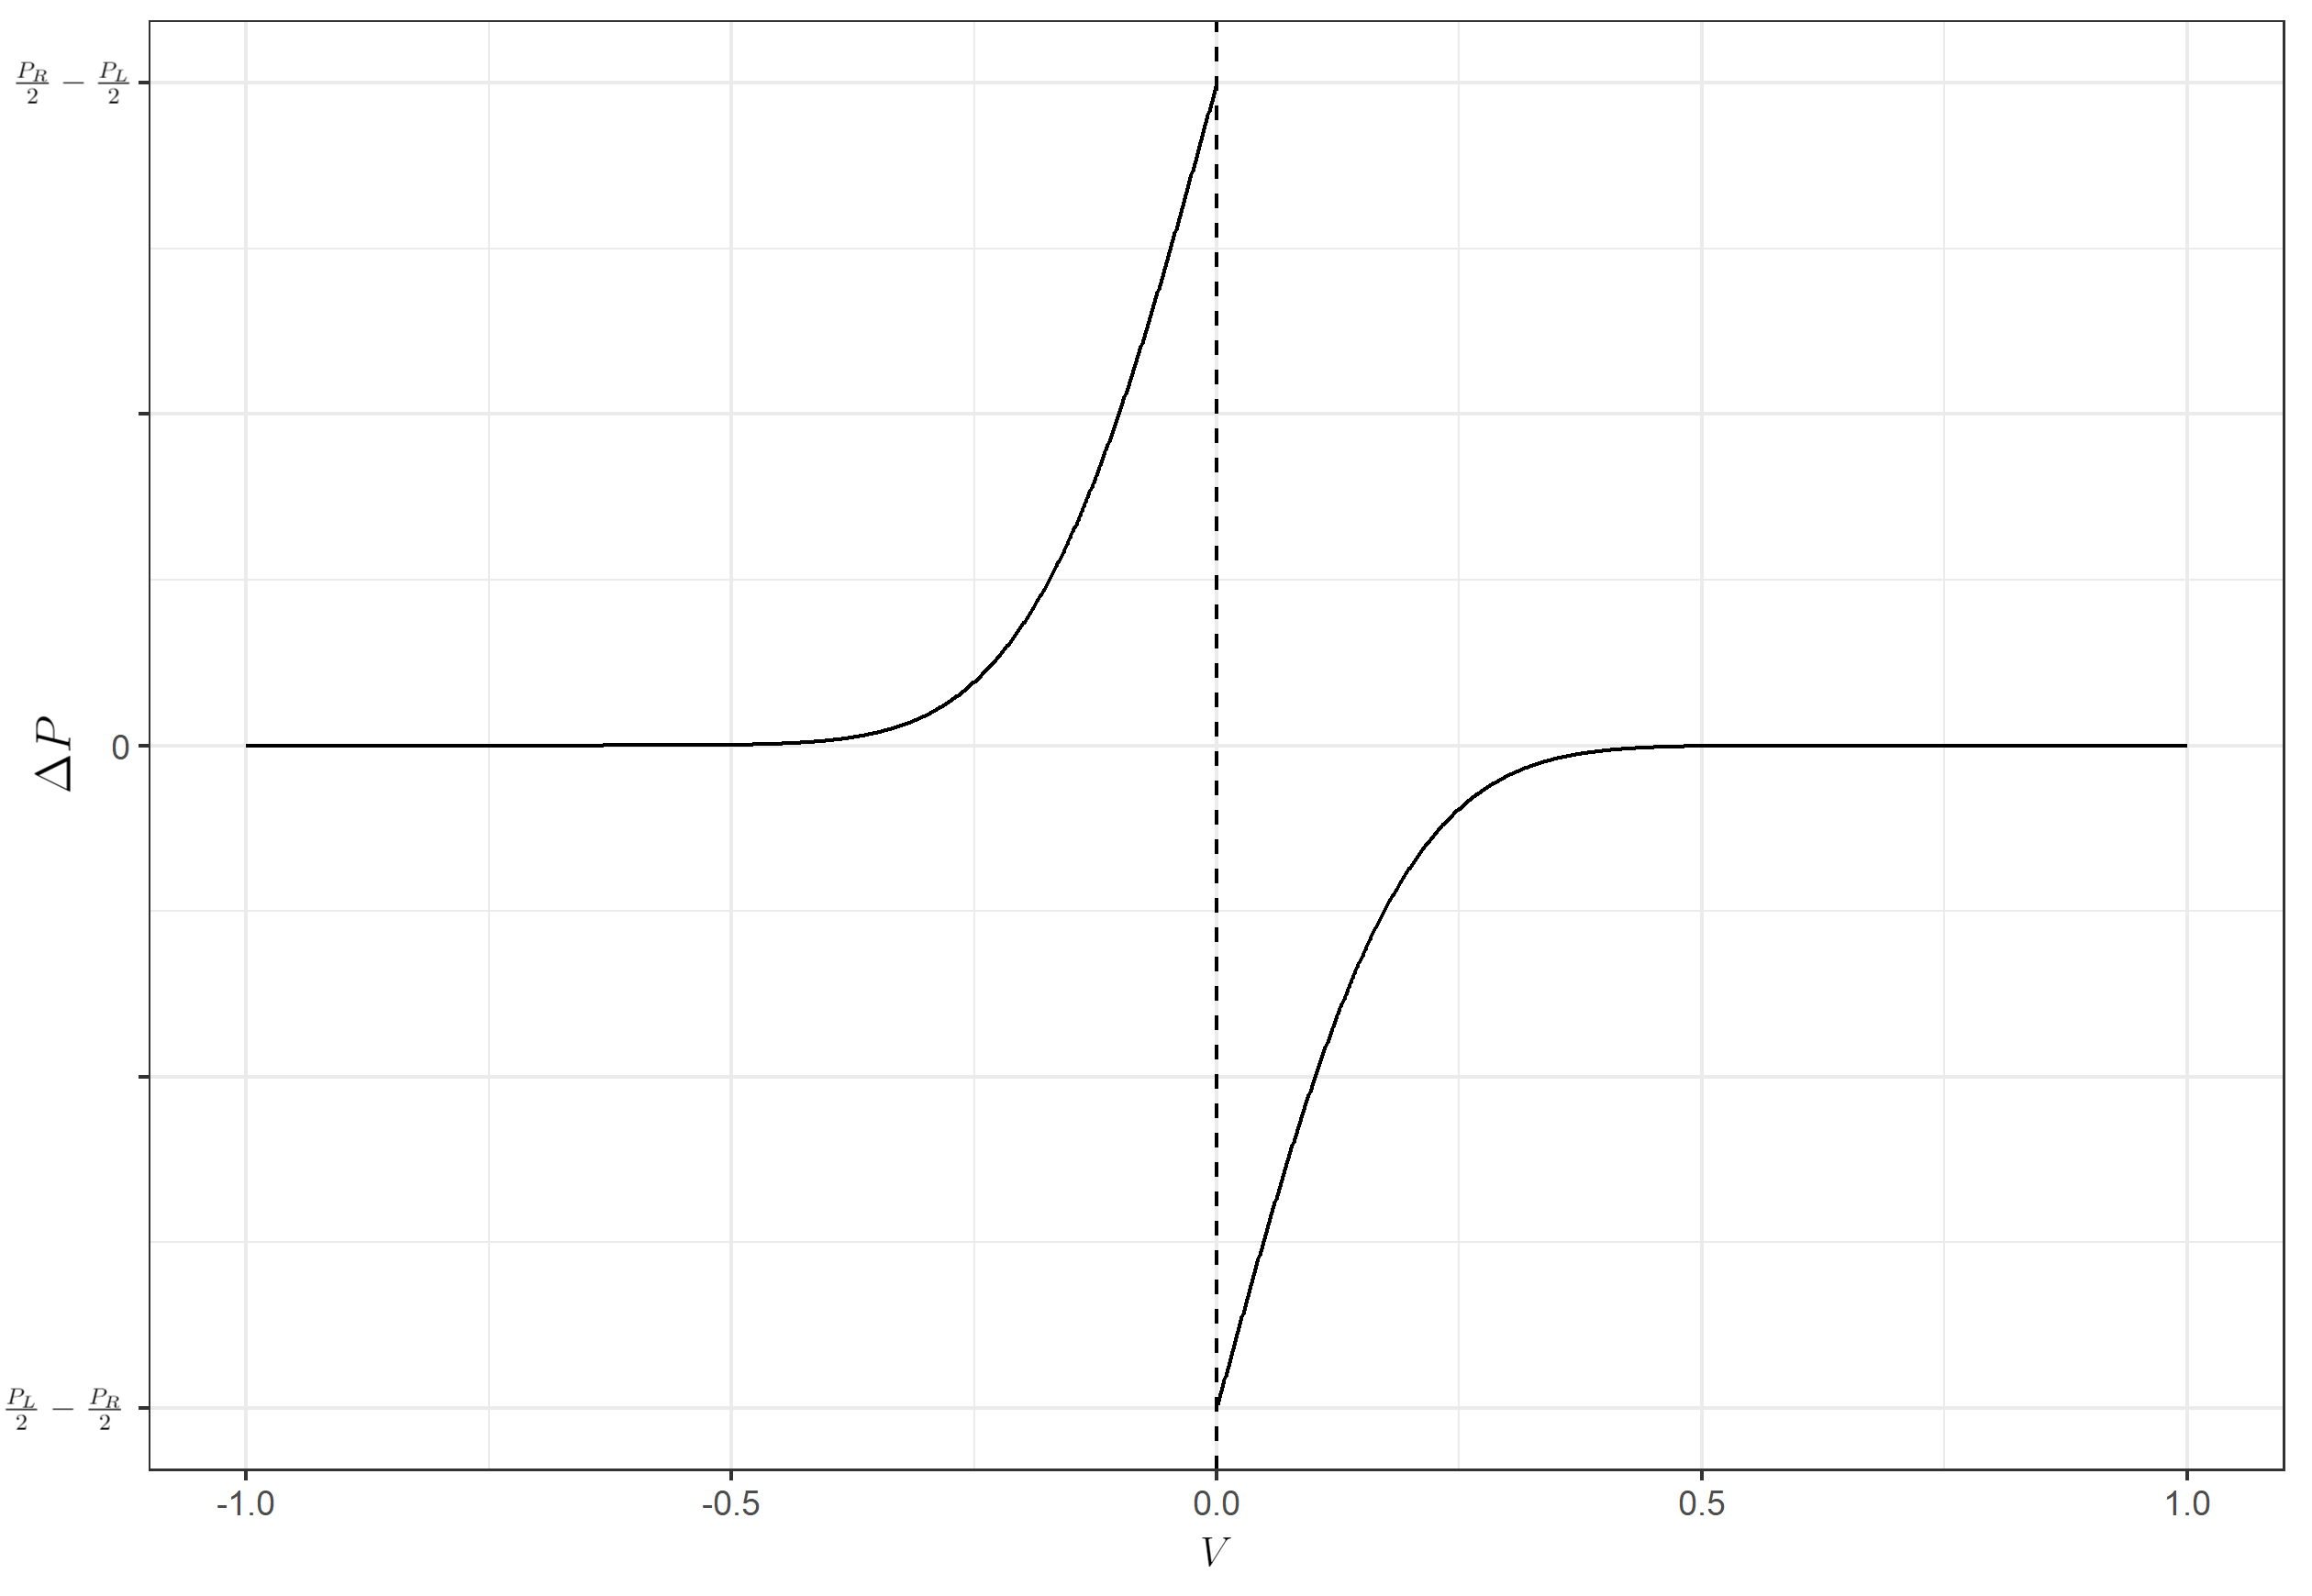
\includegraphics[width=\textwidth]{figures/Figure1.png}
    \caption{The expected shape of the conditional expectation function. Taking the difference between the two limits as they approach $V=0$ recovers the quantity of interest, $P_L - P_R$.}
    \label{fig:CEF}
\end{figure}



\section{Data} \label{section:data}

% Paragraph 14: Describe ParlGov data
Our data on parliamentary election results are from the ParlGov database compiled by \citet{Doring2018}. ParlGov contains data on parties, elections, and cabinets from all EU and OECD parliamentary democracies from 1948 to 2015. We gather from ParlGov data on each party's number of seats, the party composition of each post-election cabinet, the family classification of each party, and a 0 to 10 measure of each party's left-right ideology.\footnote{We define `Left' parties as those labeled ``Social Democracy'' or ``Communist/Socialist'' in ParlGov. ParlGov's ideology score is drawn from multiple studies estimating party ideology on a left-right scale, including \citet{Castles1984}, \citet{Huber1995}, and \citet{Benoit2006}. We assign pre-electoral coalitions the seat-weighted mean ideology score of their parties.}

% Paragraph 15: Describe adjustments for PECs
We adjust these ParlGov data to incorporate information on pre-electoral coalitions (PECs), as opposed to individual parties. PECs are sets of parties that pledge---critically: publicly, credibly, and exceedingly rarely broken---to form one government together if elected \citep{Golder2006}. Absent this information, some elections might appear close that were not (e.g., Germany's 1961 election, where SPD had a plurality, but the CDU/CSU coalition easily out-sized them), and some elections might appear lopsided that were quite close (e.g., Germany's 1976 election, where a pre-electoral coalition of SPD and FDP narrowly overtook the easily plurality Christian Democrats). For data on PECs, we rely on the dataset of \citet{Golder2006} through 1999, which we extend from primary data through 2015.\footnote{Unlike \citet{Golder2006}, our PEC data are not exhaustive. Because our analysis requires vote shares only of the largest left party and largest other party, we take particular care to identify PECs that affect these two values. These include, most prominently, the Liberal/National coalition in Australia, the CDU/CSU alliance in Germany, and the Red-Green / Centre-Right pre-electoral alliances in Sweden. We can ignore most of the more-numerous smaller-party PECs formed to overcome electoral vote-share thresholds.}

% Paragraph 16: Define forcing variable and dependent variable
For each election, we identify the largest (by seats) left party or PEC and the largest other party or PEC. We then compute the seat gap, $V$, as a percentage of these top-two parties' total parliamentary seats. The final dataset contains 576 elections, for which we were able to obtain applicable interest-rate data, our dependent variable, in 335 cases. Specifically, we use the long-term (10-year) interest rate on government bonds, reported monthly from the \citet{OECD2018} and the IMF's International Financial Statistics database \citep{IMF2018}.\footnote{We combine these sources to maximize country-year coverage, using IMF data where (rarely) they disagree. (Only Iceland exhibits any appreciable discrepancies.) All results are robust to reasonable alternative choices in these regards.} The bond market response to the election is computed by taking the difference between this rate at $t_0$ (election month) and $t_m$ ($m$ months following the election).

\section{Empirical Analysis} \label{section:results}

\subsection{Evaluating the Mechanism}

% Paragraph 17: Describe CCT estimator
Throughout our empirical analysis, we follow current state-of-the-art practices in regression discontinuity design, as suggested by \citet{Calonico2014}. This procedure (hereafter CCT) estimates two low-order local polynomial regressions (often linear) on each side of the threshold, using a triangular kernel to place greater weight on observations close to the threshold and dropping data outside of a bandwidth selected to minimize mean squared error of the RD estimator.\footnote{This procedure should be flexible enough to properly capture the theoretically expected form of the discontinuity seen in Figure \ref{fig:CEF}.} The estimated \textit{treatment effect} is the difference between the limits of these two regressions as they approach the threshold. Because this approach aims to be nonparametric (i.e., not assume a data-generating process), the CCT estimate subtracts a bias-correction term for any misspecification error in the estimation procedure and constructs robust confidence intervals centered around this bias-corrected estimate. 

% Paragraph 18: Where is the discontinuity sharp?
The first condition for validity of an RD design is that the discontinuity exists: in our application, e.g., that a left-party/PEC crossing to a seat plurality yields a discontinuous jump in the probability that left-party/PEC enters government. This assumption is easily verified directly. Figure \ref{fig:firststagefigure} shows the relationship between the largest left-party/PEC plurality margin ($V$) and its inclusion in the cabinet. The figure reveals clearly a sharper discontinuity in some countries than in others. Countries with few parties in parliament exhibit a very sharp discontinuity (left panel), whereas in countries with more-fragmented party systems, and so more potential coalitions, a left plurality is less predictive of left government. In what follows, we will define party-system fragmentation based on the Effective Number of Parliamentary Parties (ENPP).\footnote{$ENPP = \frac{1}{\sum p_i^2}$, where $p_i$ is the seat share of party $i$.} When fragmentation is low ($ENPP < 3.5$), there is a very sharp discontinuity at the plurality threshold, but where high ($ENPP > 3.5$), there is no statistically significant discontinuity (see Table \ref{table:firstStageRD}).\footnote{Henceforth, we use this threshold ($ENPP = 3.5$) as the cutoff between Low and High party fragmentation. Appendix \ref{appendix:robustness}, demonstrates that the results are robust to this choice. Appendix \ref{appendix:robustness} also lists the country-years above and below this cutoff. Note that the Low Fragmentation countries are not exclusively majoritarian countries with single-party governments; they include some countries with proportional representation (e.g., Spain and Portugal) and some with coalition governments (e.g., Germany).} Because there is no discontinuity in high-fragmentation party-systems, we can use this set of countries as a sort of placebo group. A narrow plurality for left parties should only cause market reactions if it provides new information about government formation. In high-fragmentation countries, it does not, so we should not expect to observe discontinuous bond-price movements in those countries. 



\begin{figure}[h]
\centering
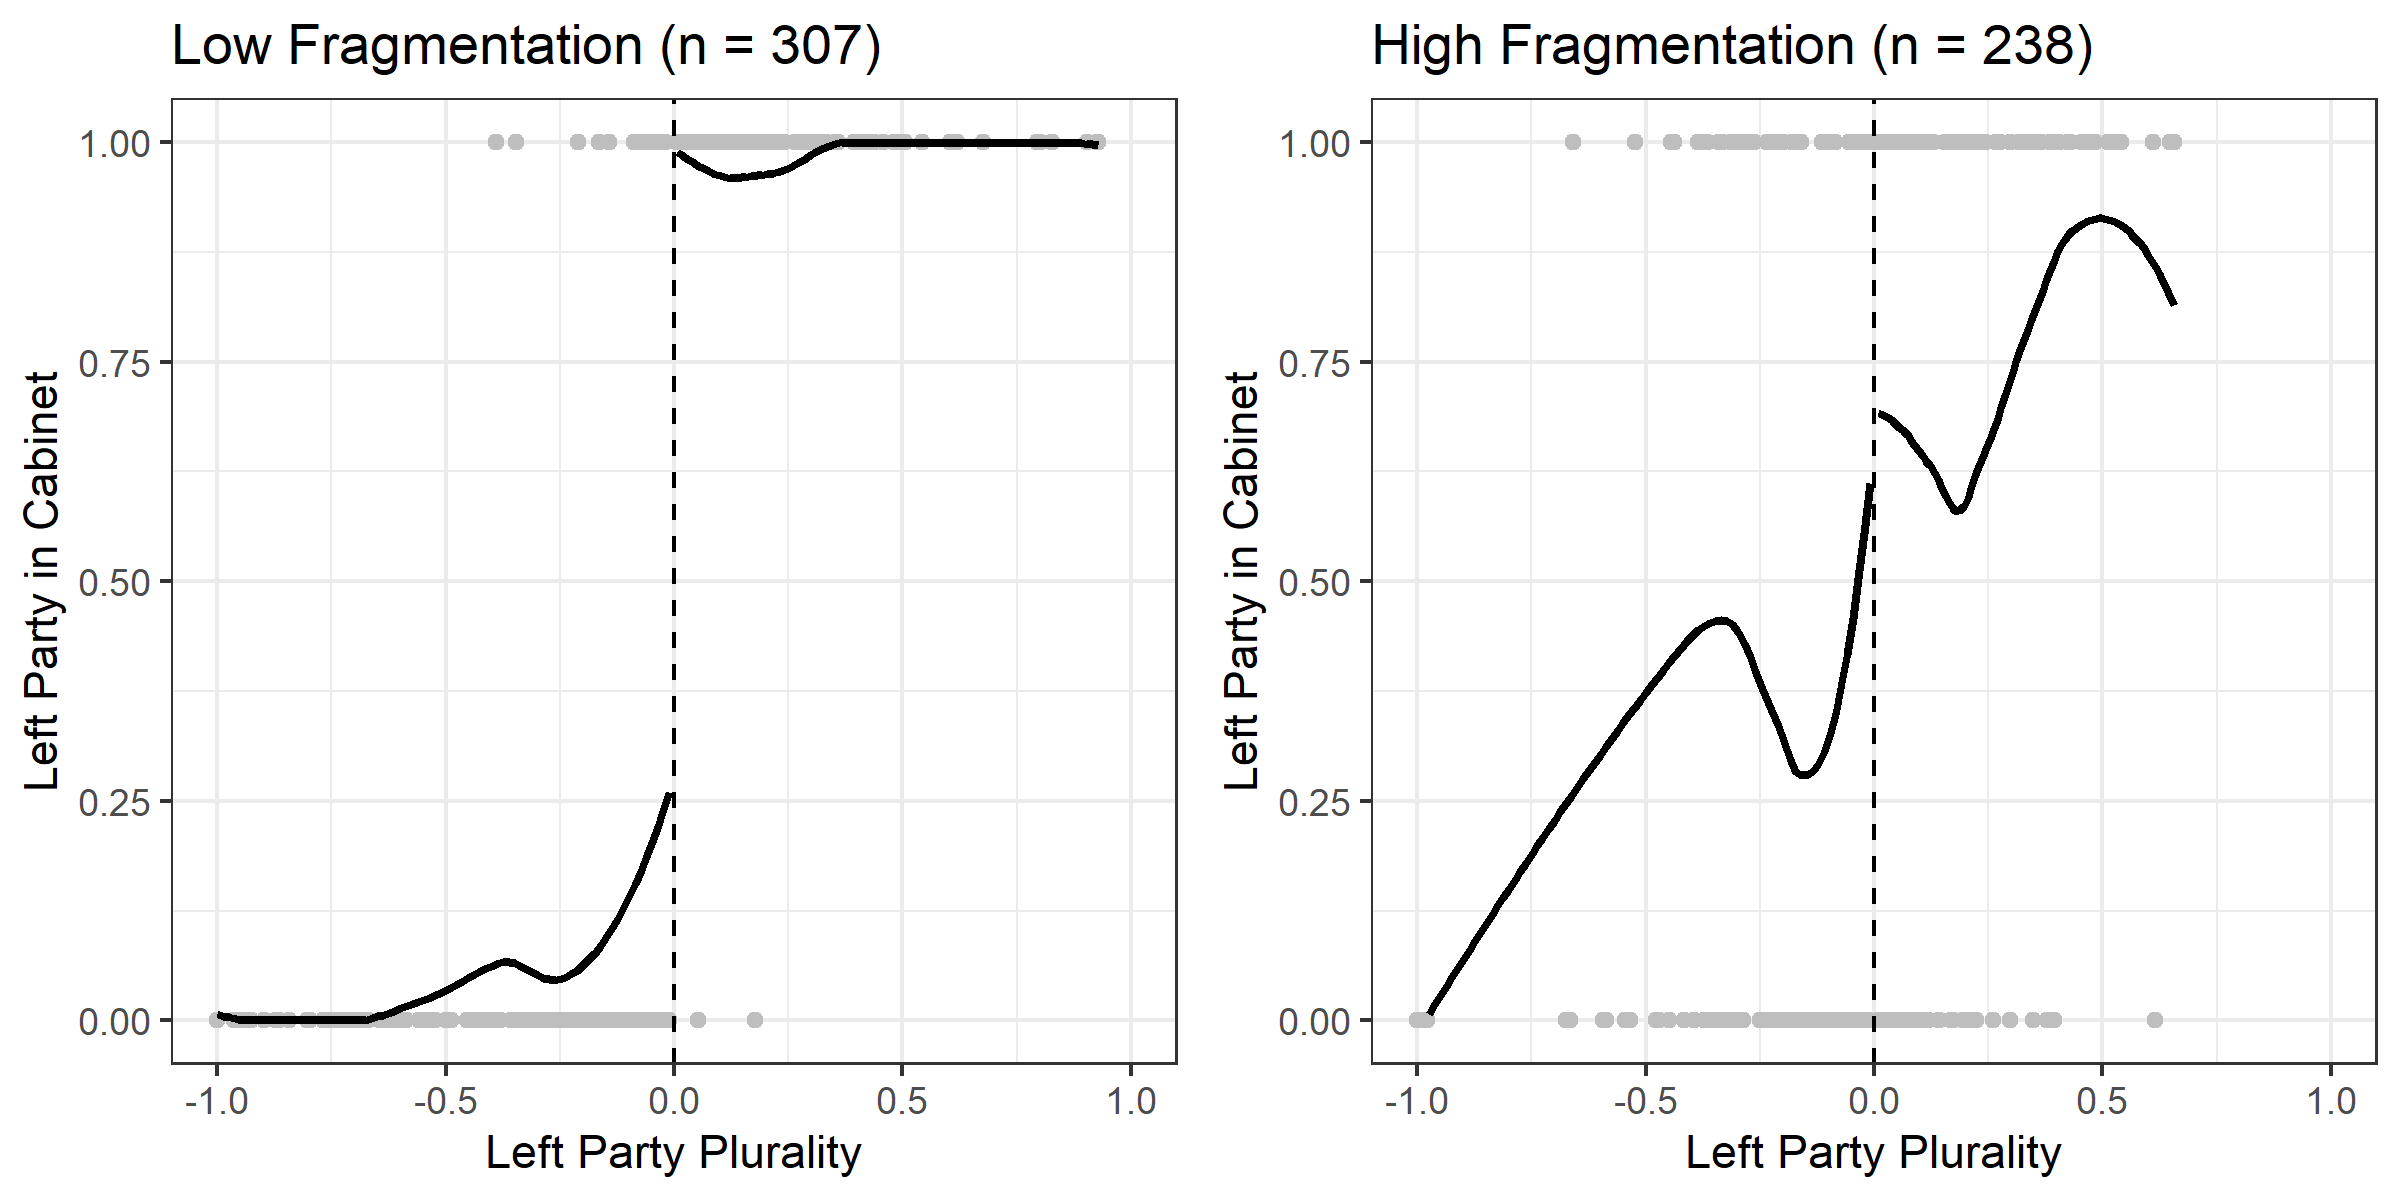
\includegraphics[width=\linewidth]{figures/Figure2.png}
\caption{Left party plurality plotted against binary indicator of left party entering cabinet; curves are LOESS fits. Where party-system fragmentation is low ($ENPP < 3.5$), there is a sharp discontinuity in the probability of left parties entering government as they achieve a plurality of seats in parliament. Where party-system fragmentation is high ($ENPP > 3.5$), there is no such discontinuity.}
\label{fig:firststagefigure}
\end{figure}



% Table created by stargazer v.5.2.2 by Marek Hlavac, Harvard University. E-mail: hlavac at fas.harvard.edu
% Date and time: Fri, Nov 16, 2018 - 2:02:49 PM
\begin{table}[h] \centering 
  \caption{First-stage regression discontinuity estimates (bias-corrected) with 95\% confidence intervals (robust standard errors) in brackets.} 
  \label{table:firstStageRD} 
\begin{tabular}{@{\extracolsep{5pt}}lccc} 
\\[-1.8ex]\hline 
\hline \\[-1.8ex] 
 & \multicolumn{3}{c}{\textit{Fragmentation:}} \\ 
\cline{2-4} 
\\[-1.8ex] & All & Low & High \\ 
\\[-1.8ex] & (1) & (2) & (3)\\ 
\hline \\[-1.8ex] 
 Local Average Treatment Effect & 0.233 & 0.575 & 0.037 \\ 
  & [-0.035, 0.50] & [0.35, 0.80] & [-0.35, 0.42] \\ 
\hline \\[-1.8ex] 
Observations & 551 & 309 & 242 \\ 
Observations Within Bandwidth & 256 & 158 & 127 \\
Bandwidth $(h)$ & 0.175 & 0.218 & 0.181 \\ 
\hline 
\hline \\[-1.8ex] 
\end{tabular} 
\end{table} 


\subsection{Balance Tests}

% Paragraph 19: Balance Tests
A crucial identifying assumption for the RD design is that the treatment must be the only variable that changes discontinuously at the threshold. If any other covariates do so as well, then one cannot unequivocally attribute a discontinuity in the outcome to the treatment alone. We subject a number of pre-treatment covariates to tests of this continuity condition. For each covariate, we estimate a local-linear RD (triangular kernel), testing whether the difference in expected value on either side of the threshold differs significantly from zero. The covariates we test include GDP per capita, Polity score, population, central government debt per capita, government expenditures, tax revenue per capita, annual inflation, and OECD average bond yields. The latter test serves to ensure that our main results are not being driven by global movements in the bond market, but by country-specific bond price changes. 

% Paragraph 20: Balance Test Results
Figure \ref{fig:balanceplots} uncovers no significant discontinuities for any of these covariates, except government expenditures; after elections yielding slight left-party pluralities, central government expenditures as a percent of GDP are slightly \textit{lower}. Although this seems unlikely to be the cause of a discontinuity in bond-yield \textit{changes}, a robustness check considered in Appendix \ref{appendix:robustness} deploys a variant of the RD estimator that conditions on covariates, as proposed by \citet{Calonico2018}. These conditional-RD results are very similar to those in the primary analysis.

\begin{figure}
\centering
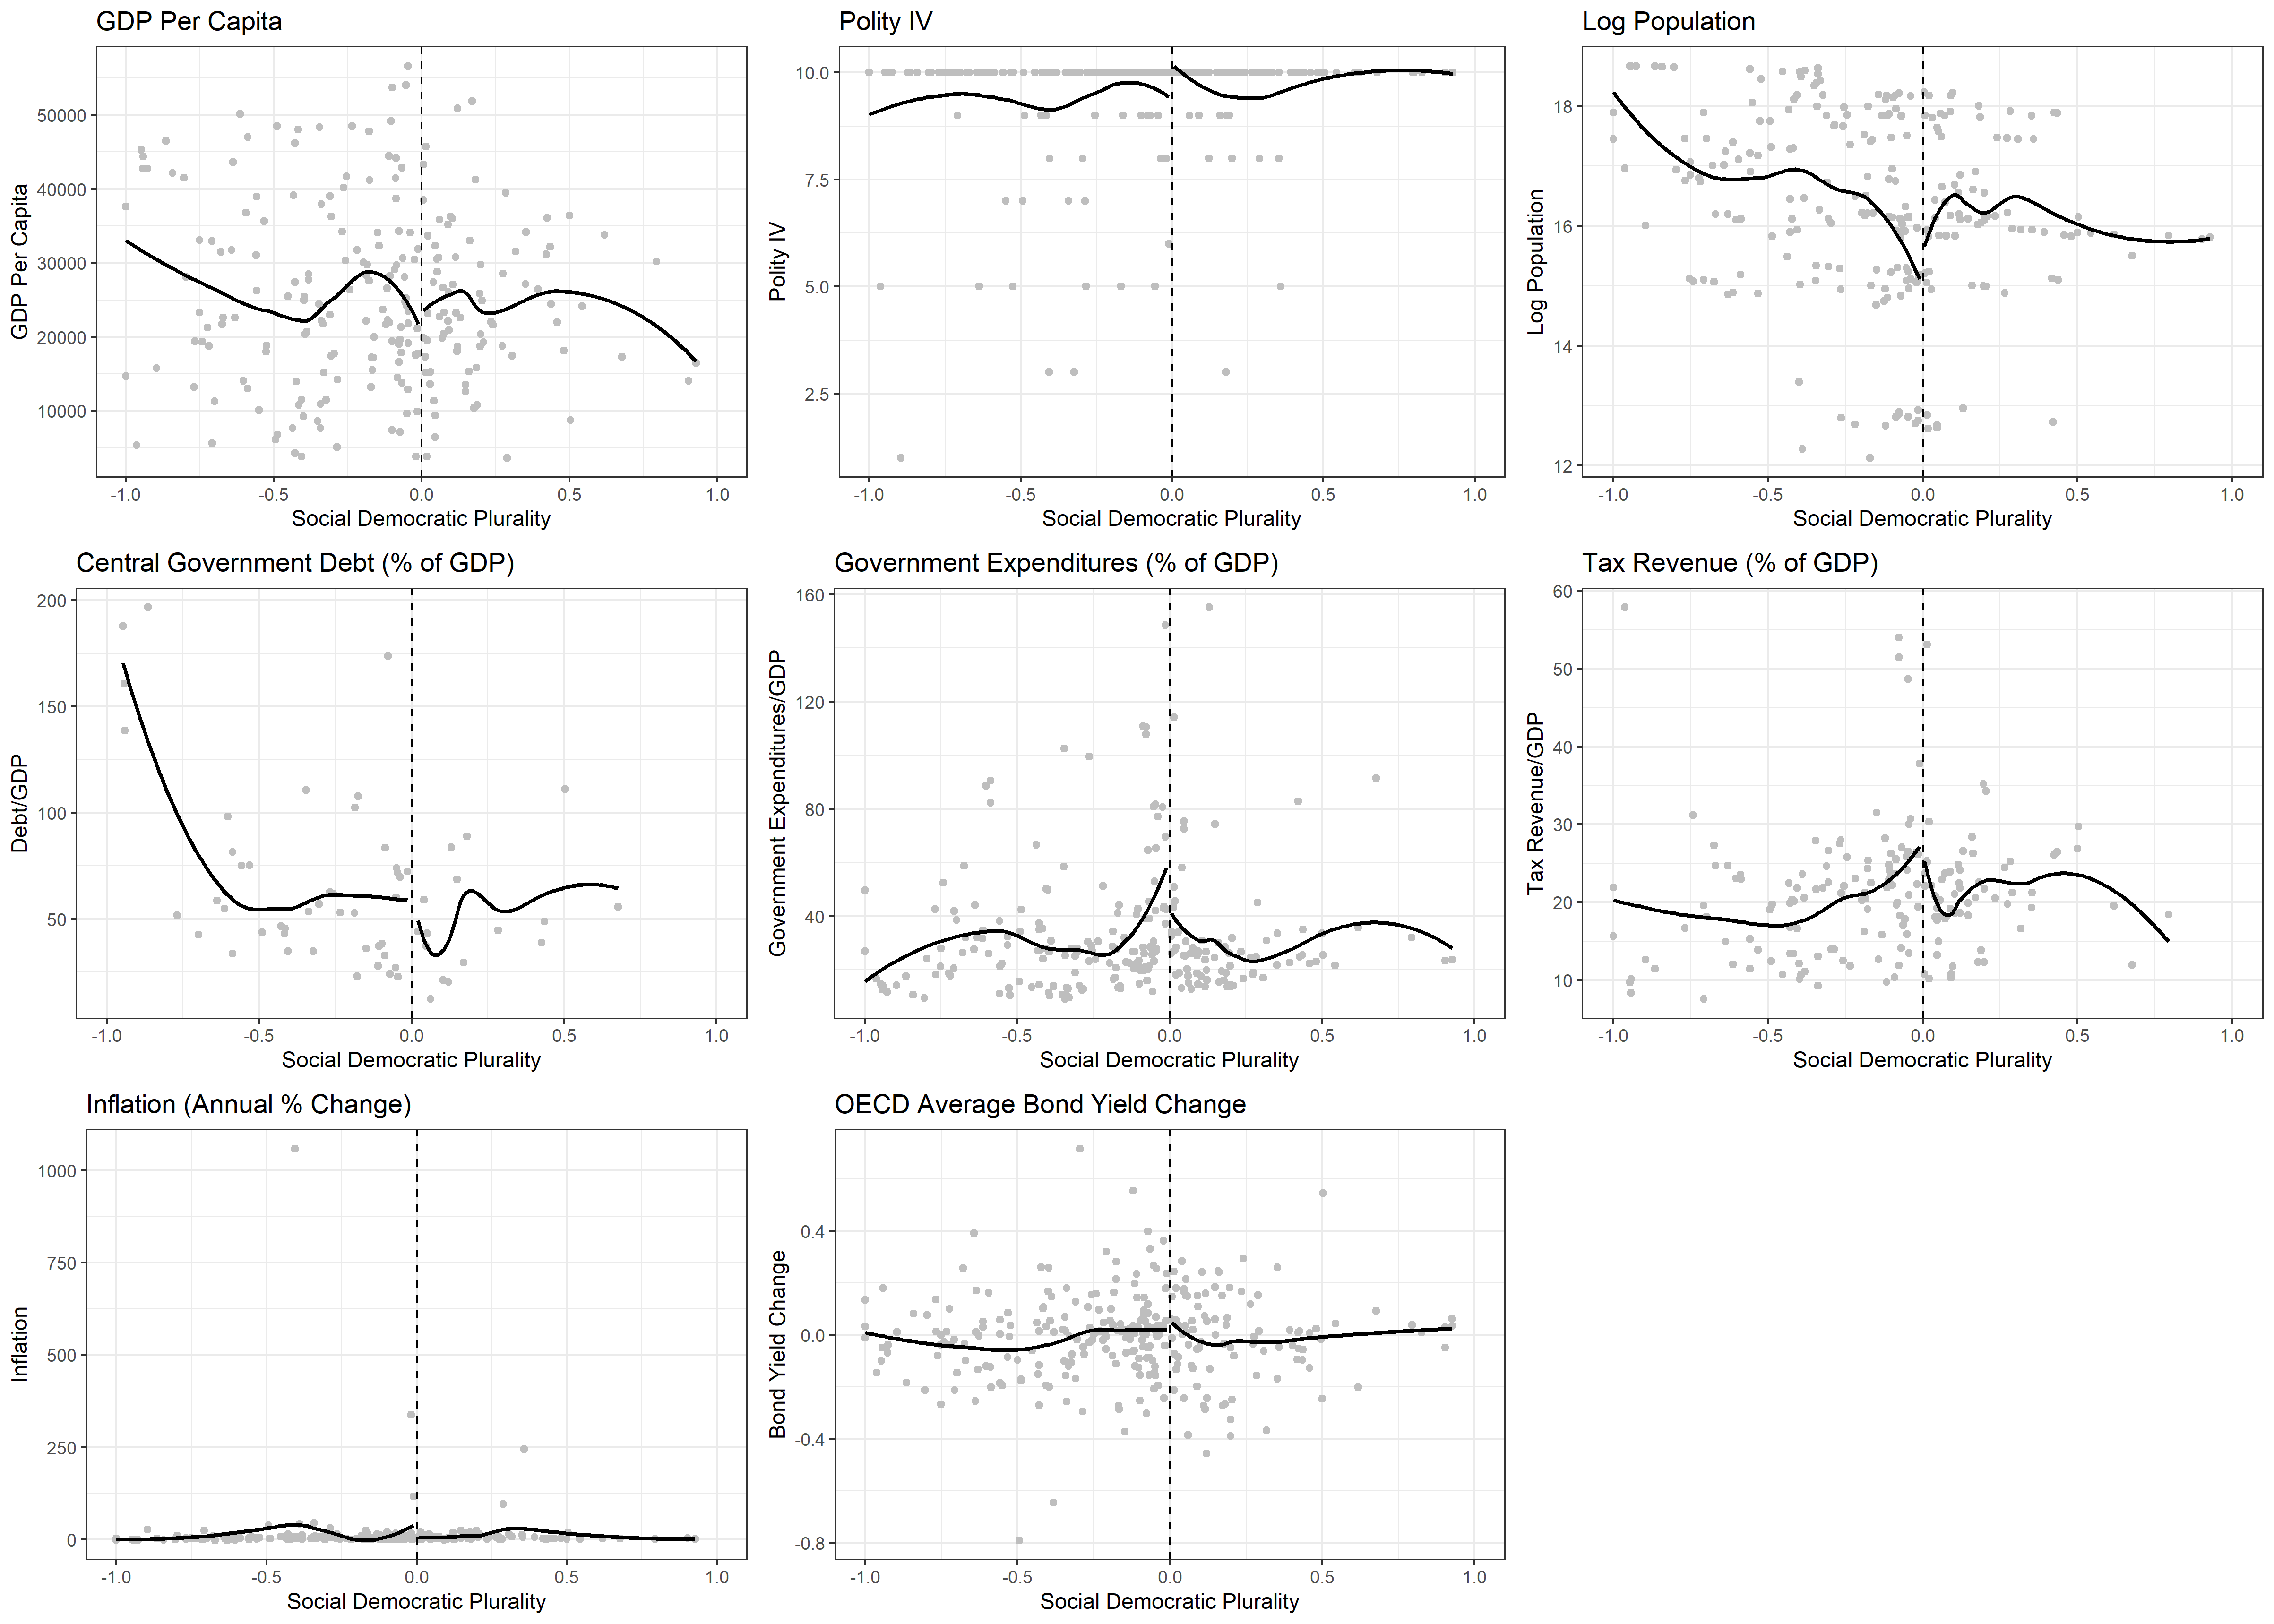
\includegraphics[width=\linewidth]{figures/Figure3.png}
\caption{For nearly every pre-treatment covariate, there is no significant discontinuity at the threshold. Note that these tests are conducted for elections with low party fragmentation, as in the primary analysis, but the finding holds when looking at the entire sample as well.}
\label{fig:balanceplots}
\end{figure}

\subsection{Bond Markets}

% Paragraph 21: LATE estimates, varying fragmentation
Table \ref{table:InterestRateRD} reports, and Figure  \ref{fig:interestraterdfigure} illustrates, the estimated Local Average Treatment Effect (LATE) of left-party entry to government following closely contested winning of parliamentary plurality, in samples of high party-system fragmentation, in low-fragmentation systems, and in all systems. In High-Fragmentation ($ENPP > 3.5$) countries, we see no statistically significant discontinuity in bond yields at the threshold. In these contexts, left-party involvement in government does not seem to bring higher government-bond interest-premia costs, perhaps because governments therein tend to be multiparty and so inertial. In contrast, in Low Fragmentation ($ENPP < 3.5$) countries, there is a roughly half-a-percentage-point increase in bond yields one month after a left party narrow plurality win. Precisely as our mechanism predicts, and striking in magnitude: left-party government, at least in low-fragmentation contexts where governments tend to be relatively efficacious single- or few-party majorities, are estimated to ``cost'' roughly half a percentage point higher interest-premia on government debt! Finally, with the benefit of comparison of results from low-fragmentation and high-fragmentation samples, the entire-sample LATE estimates can be seen as influenced by these heterogeneous-treatment effects to suggest only a marginally insignificant interest-rate increase less-than one-quarter as large as that in low-fragmentation contexts (and the whole-sample estimate is about 85\% noisier proportionately to effect-size).

% Table created by stargazer v.5.2.2 by Marek Hlavac, Harvard University. E-mail: hlavac at fas.harvard.edu
% Date and time: Fri, Nov 16, 2018 - 2:02:49 PM
\begin{table}[ht] \centering 
  \caption{1-month bond yield regression discontinuity estimates (bias-corrected) with 95\% confidence intervals (robust standard errors) in brackets.} 
  \label{table:InterestRateRD} 
\begin{tabular}{@{\extracolsep{5pt}}lccc} 
\\[-1.8ex]\hline 
\hline \\[-1.8ex] 
 & \multicolumn{3}{c}{\textit{Fragmentation:}} \\ 
\cline{2-4} 
\\[-1.8ex] & All & Low & High \\ 
\\[-1.8ex] & (1) & (2) & (3)\\ 
\hline \\[-1.8ex] 
 Local Average Treatment Effect & 0.145 & 0.592 & $-0.048$ \\ 
  & [-0.12, 0.41] & [-0.01, 1.19] & [-0.32, 0.23] \\ 
\hline \\[-1.8ex] 
Observations & 316 & 179 & 137 \\ 
Observations within Bandwidth & 135 & 70 & 63 \\
Bandwidth $(h)$ & 0.137 & 0.141 & 0.125 \\ 
\hline 
\hline \\[-1.8ex] 
\end{tabular} 
\end{table}  

\begin{figure}[h]
\centering
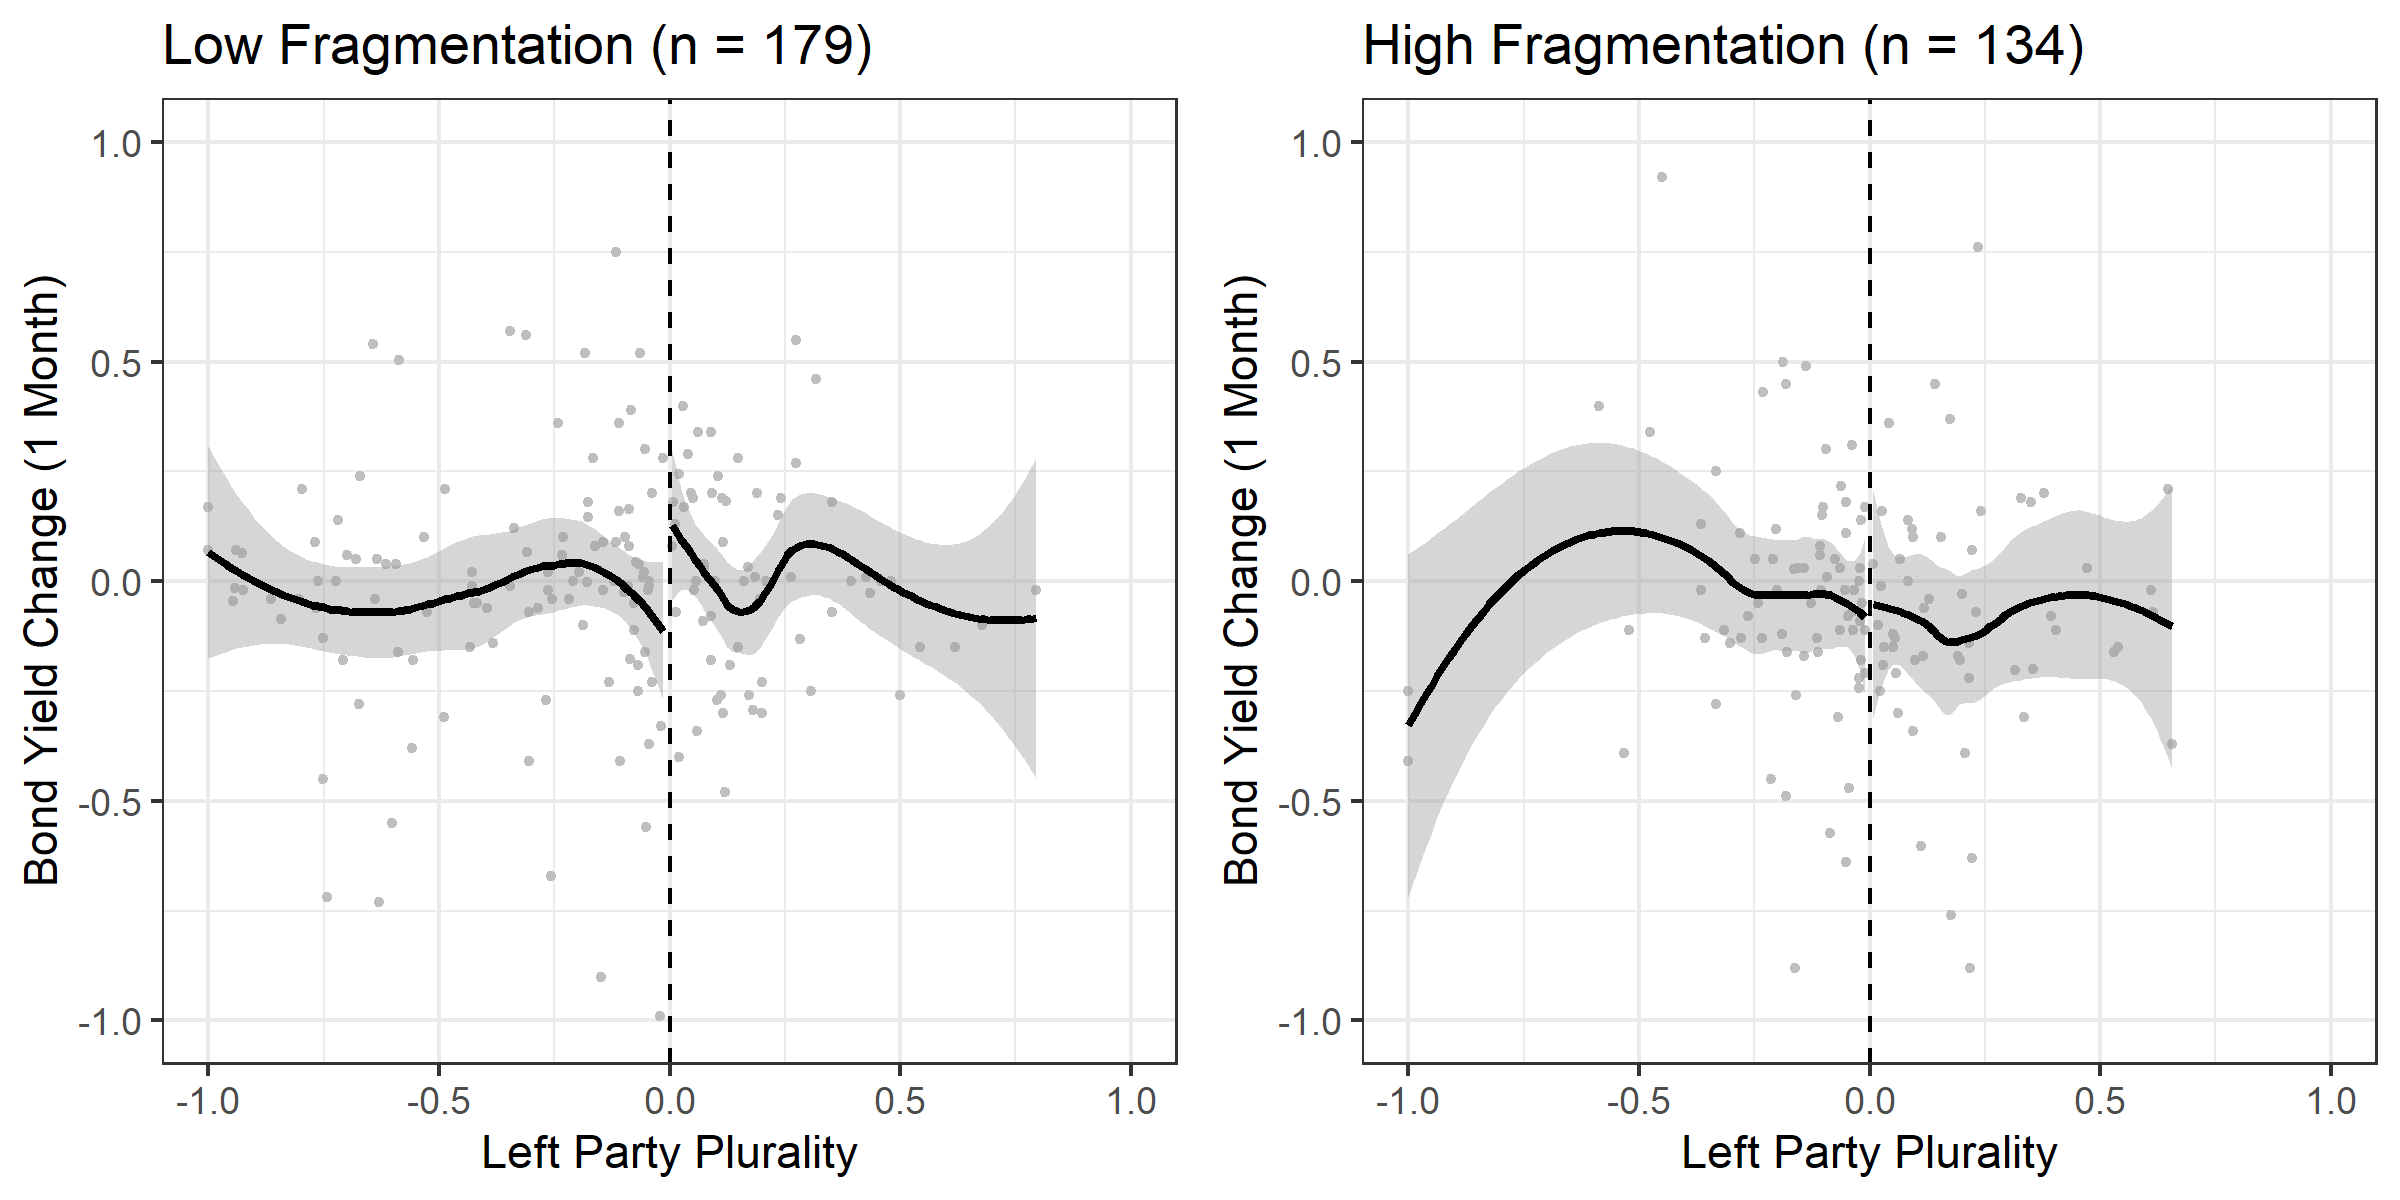
\includegraphics[width=\linewidth]{figures/Figure4.png}
\caption{Interest rate change 1 month after election, plotted against the plurality margin of the largest social democratic party; curves are LOESS fits.}
\label{fig:interestraterdfigure}
\end{figure}


\subsection{Further Exploration of Heterogeneous Treatment Effects}

% Paragraph 22: Hetergeneous TFX 1: Ideological Distance
The strength of the bond-market response to left government likely depends on the counterfactual, namely, in this context, on how far that left government is from the alternative that \textit{would} have formed had the left not gained plurality. We would expect bond-market movements to be strongest when the party that lost the plurality was strongly conservative relative to a strongly left party that won it. Whereas, if both parties vying for the plurality were broadly parties of the center-left, then the election outcome would have revealed little information to financial markets about likely bond-price relevant policies of the new government: bond prices would hardly move. To explore this hypothesis, we test how the RD estimate varies with the absolute difference between the plurality-contending parties' ParlGov ideology score.\footnote{In so doing, we sacrifice some of the nonparametric character of our design to gain further insight (and efficiency and precision) by using these \textit{measures} of ideology.} Figure \ref{fig:rdEstimateVaryingIdeologyDistance} plots these estimates, showing further evidence that the treatment effect arises from the information-revelation that occurs when a left party narrowly gains plurality status: the LATEs are clearly larger when we restrict the sample to cases where the absolute difference in ideology score is large (e.g., greater than 3).\footnote{A caveat, however: the sample sizes for those estimates are relatively small ($n = 69$).}

\begin{figure}[h]
	\centering
	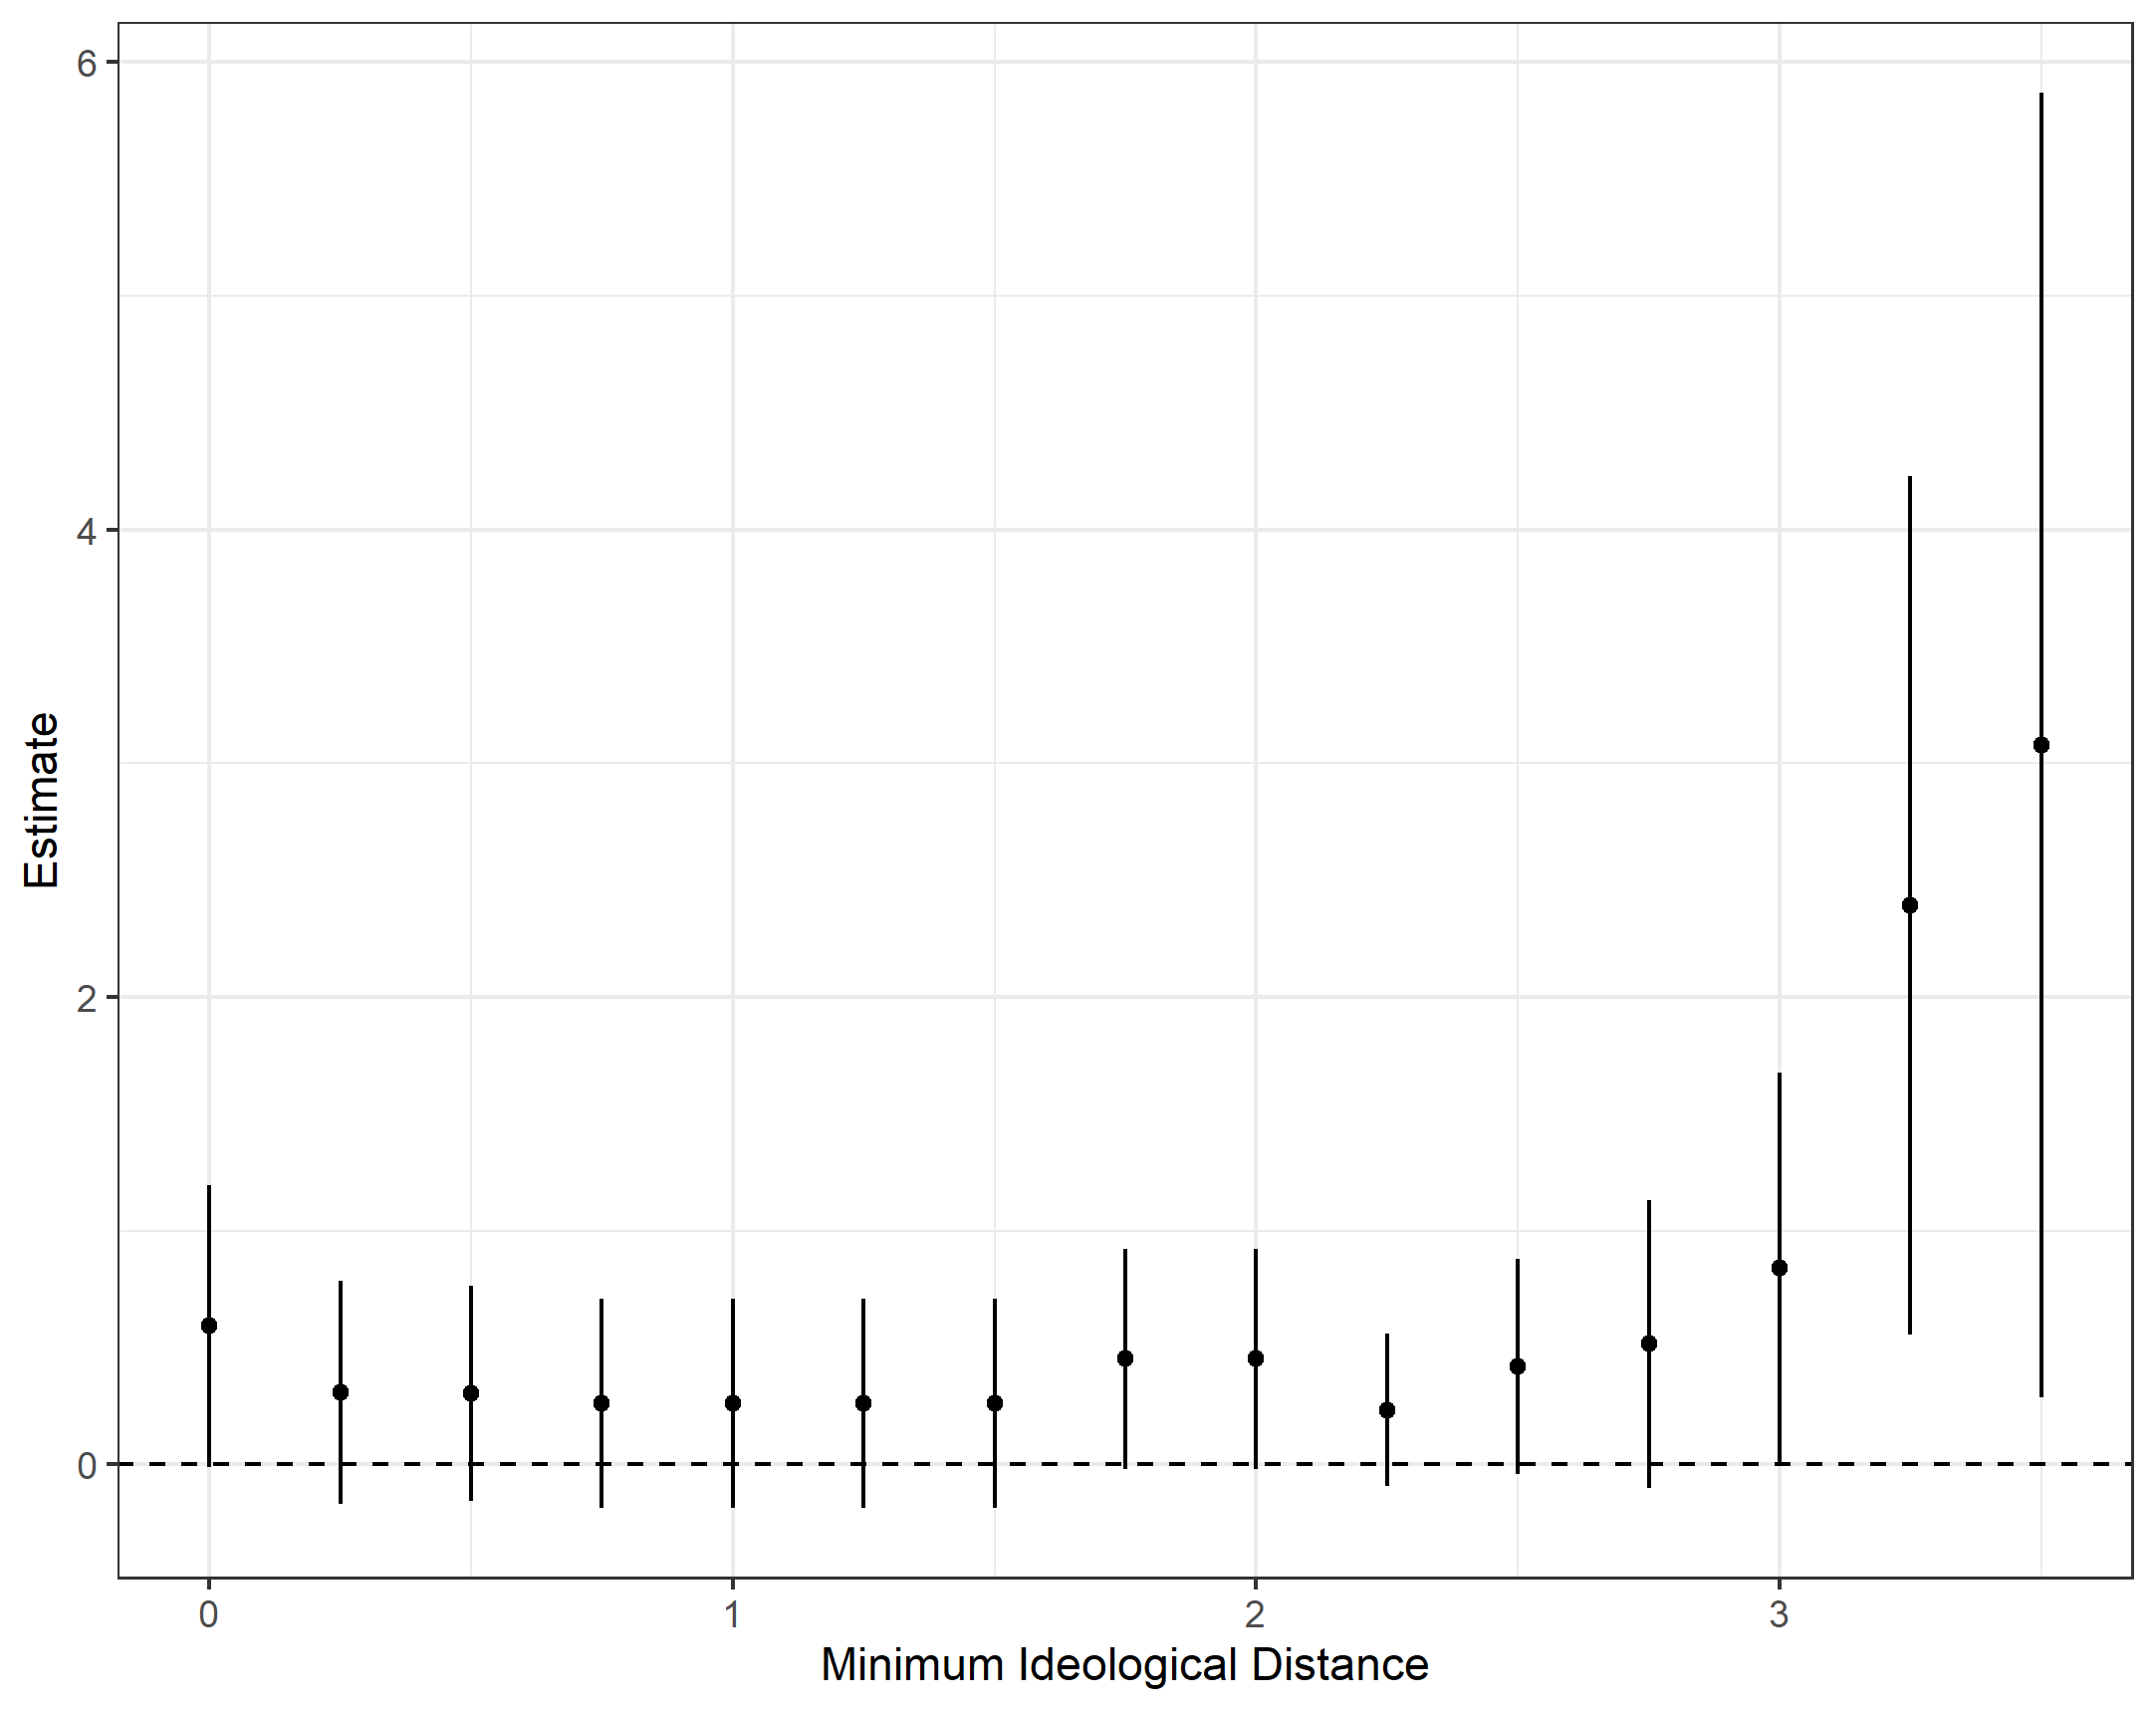
\includegraphics[width=\linewidth]{figures/Figure5.png}
	\caption{When we restrict our estimates to elections where the two largest parties are ideologically distant, the estimated treatment effect grows.}
	\label{fig:rdEstimateVaryingIdeologyDistance}
\end{figure}

% Paragraph 23: Heterogeneous TFX 2: Historical Era
Figure \ref{fig:rdEstimateVaryingYear}, lastly, illustrates how the estimated LATE varies over time; each plotted point reports an estimate and confidence interval from a 30-year window of data starting from the year indicated on the X-axis. Interestingly, the interest-rate effect of left government is largest and most discernible around the Bretton Woods era of fixed exchange-rates and low capital-mobility (from early 1950s through mid-to-late 1970s). This would be consistent with Rodrik's ``golden straightjacket'' hypothesis -- i.e., with considerable globalization-and-capital-mobility constraint on domestic governments' policymaking autonomy, \textit{if} the reason we are not finding interest-rate effects of left government in the later period is because their policies do not (or are not expected to) differ much from other governments. After all, furthermore, Mundell-Fleming suggests that monetary and fiscal policy should have been at least moderately maneuverable and effective in that 1950s-1970s era of limited capital-mobility and (so) \textit{imperfectly} fixed exchange-rates; and both monetary and fiscal policy should have grown less maneuverable and/or effective as capital grew highly mobile and the remaining dependent central banks increasingly independent (although exchange-rate-fixing efforts lessened this straight-jacketing some for a time) \citep{Clark2003, Franzese2003}.

\begin{figure}
\centering
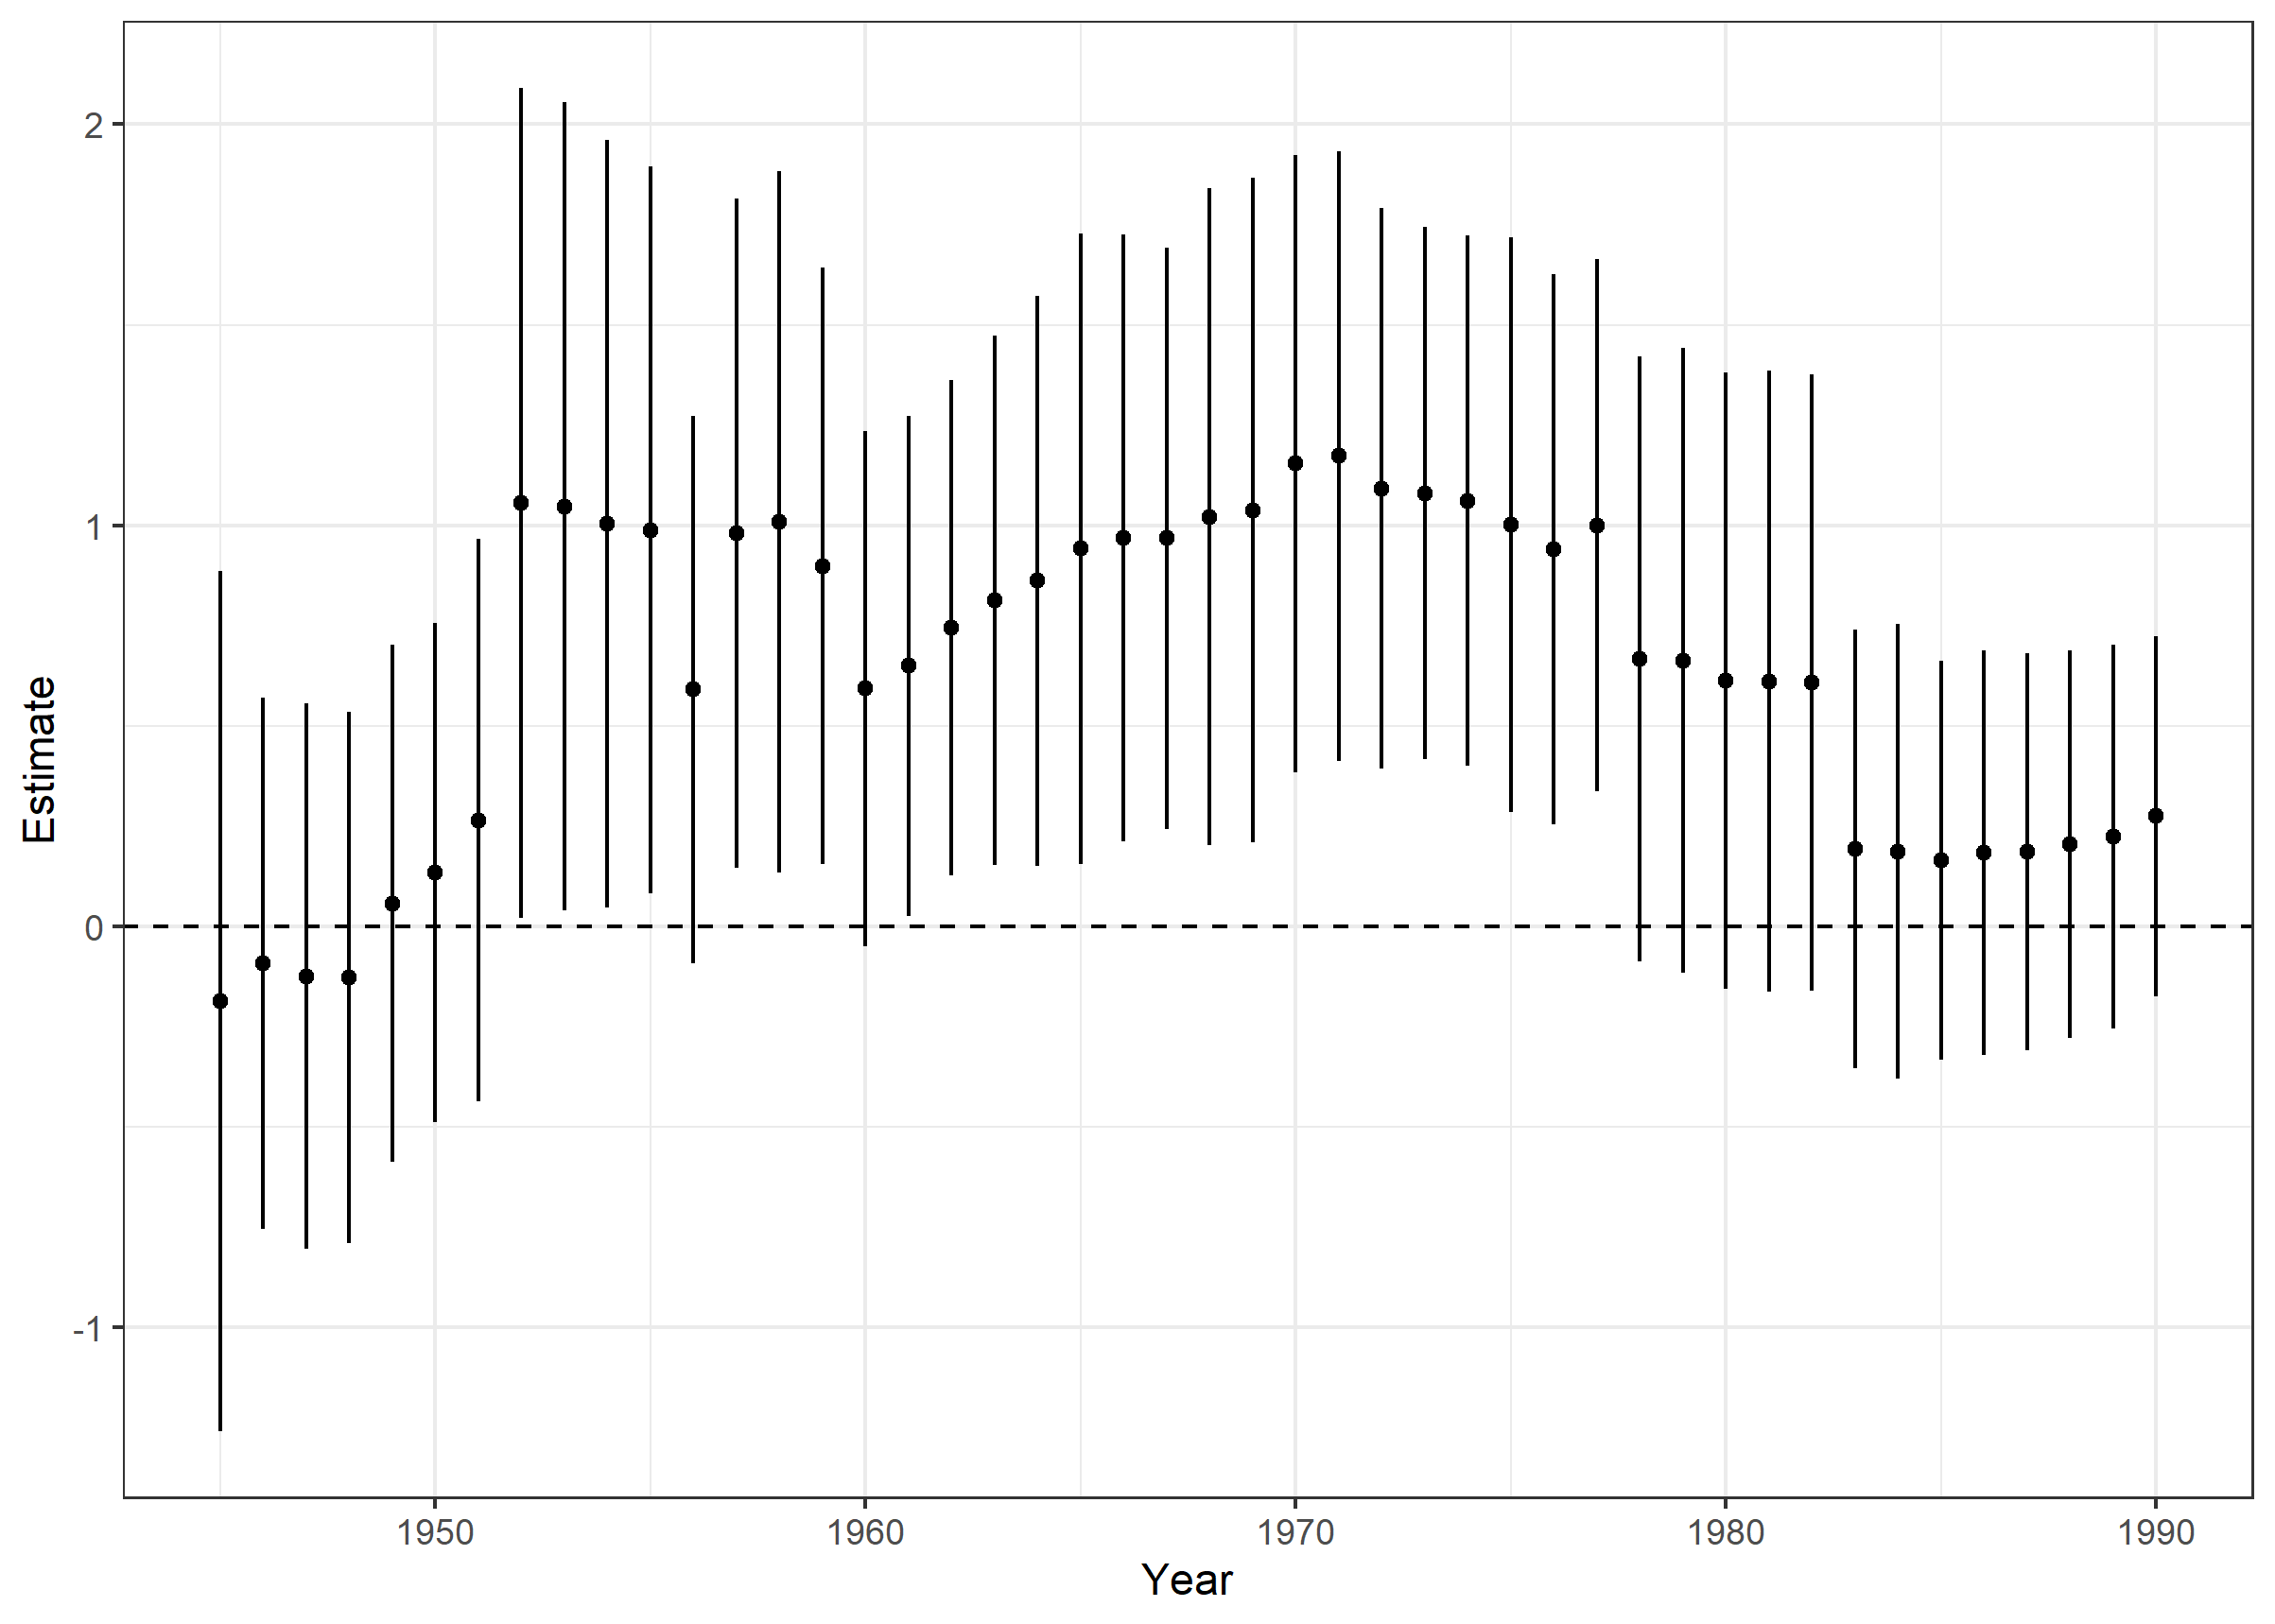
\includegraphics[width=\linewidth]{figures/Figure6.png}
\caption{RD estimates and 95\% confidence intervals, varying the time period of analysis. (Each point is estimated using 30 years of data; x-axis denotes the minimum year.)}
\label{fig:rdEstimateVaryingYear}
\end{figure}

\section{Conclusion}

% Paragraph 24: Summarize Results
A discontinuous increase in the probability of a party's entry to government at the  parliamentary seat plurality threshold offers quasi-experimental identification of the causal effect, in that plurality-threshold vicinity, of that party on outcomes we think it may influence in government. We focused on the interest-rate-premium cost of left-party government that financial markets add to government-bond yields.\footnote{% Paragraph 25: Limitations and Future Work
Some important limitations and potential pitfalls to our approach merit mention. One issue surrounds our reliance on an \textit{ex post} measure of \textit{ex ante} uncertainty. We used an \textit{ex post} measure of how uncertain was the election outcome---how close to 50-50 was the proposition of left-party being largest---whereas the actually relevant concept for market reaction is how \textit{surprisingly} left was the government. To construct such an \textit{ex ante} measure of government-partisanship surprise, we would need pre-election polls or forecasts and party partisanship measures across our entire sample of country-years, and some manners of translating those to expectations, and a mapping from party to government partisanship; and each of these components would require further structural specifications. We believe our approach goes as far as possible, insofar as we wish to retain non-parametric causal-inference robustness over structural-specification efficiency. Moreover, we are confident our \textit{ex post} measure of electoral uncertainty is at least unbiased with respect to \textit{ex ante} electoral uncertainty. Some forecasted-close elections are landslides and some forecasted landslides are close, but both are rare and orthogonally random. Another limitation is the small number of close elections. We count 95 close elections (ones with top two parties' seat-differentials below $\pm$10\% so a 5\% swing would swap winners) in parliamentary democracies 1948-2015, and we have bond yields for only 49 of those contexts. Even this relatively small sample-size, however, proved adequate given the large market reactions at the threshold in low fragmentation, stark alternative contexts. Null results, conversely, should be viewed with these same small-sample and low-power considerations in mind. Finally, we must pool countries with widely disparate institutions and draw cases from an extended historical period. Although such broad pooling is common practice in comparative political economy, it does entail complications \citep{Beck1995}. Pooling majoritarian and proportional parliamentary democracies, e.g., may mask consequential other differences beyond that the former tend to produce single-party left and right governments whereas the latter tend to produce coalition governments on both sides. We explored this latter directly across our broad pool of democracies, saw that it generated heterogeneous effects, and we highlighted the important implications and complications arising from this heterogeneity. Other bases for heterogeneous effects may also occur across this wide diversity of parliamentary democracies. Unaccounted treatment heterogeneity, akin to specification error, induces inefficiency at best (if the heterogeneity is unrelated to treatment) and bias at worst (if related).} Applying a regression discontinuity design to this question of the (interest-rate) ``cost of left government'', and various refinements of it, we estimated that left government indeed carries quite sizable interest-rate costs, over 0.5 percentage points, in the short term---for about a year or a little more, peaking around 10 months---under certain conditions---when party-system fragmentation is low, so that (we suspect) government alternation tends to be between relatively distant left and right single- or few-party majority-government alternatives. Contrarily, such clearly discernible and appreciable interest-rate effects do not materialize in more-fragmented party-system contexts, because (we suspect) there government alternation is not as stark in ideological-distance terms and bare-plurality left parties tend to be entering multiparty and/or minority, and so more-inertial, governments. Also, we found the time window when these notable interest-rate costs of left governments in low-fragmentation systems arose was limited to around the Bretton Woods era, from the early 1950s through the mid-to-late 1970s, when capital mobility was limited and exchange rates were imperfectly fixed (among our sample countries, \textit{de facto}, to the (extra-sample) U.S. dollar). Under these prevailing conditions, autonomous domestic government monetary and fiscal policy maneuverability and efficacy was relatively high. As these (and other: e.g., high and rising central-bank independence) conditions changed, domestic-government policy autonomy, maneuverability, and efficacy will have faded, which could explain the reduced magnitude and certainty of left interest-rate cost estimated in later periods. To explore how accurate are our interpretations of the varying interest-rate costs of left government that we estimated in low-fragmentation \textit{versus} high-fragmentation contexts, in contexts of starker partisan alternation across governments, and over the moving-window estimates showing sizable and discernible effects only in the 1950s through 1970s period of, perhaps, relatively greater domestic-government policy autonomy, future analyses should explore bond-relevant economic-policy differences near the discontinuity. Are there differences in policy that could explain the variation in the estimated interest-premium effects corresponding to differences in domestic and international political-economic institutions and structure that we suggest are driving these heterogeneous effects we discovered? \textit{Inter alia}, these analyses will help distinguish whether we are observing Downsian convergence in policies due to democratic competition and so in financial-market outcomes; convergence in policies and outcomes from globalization-induced policy competition; convergence in outcomes but not in policy, indicating lack of market concern about those policies or suggesting some non-policy-related market reaction to left government; and/or some other political-economic institutional-contextual conditioning of partisan-government effects on policy and/or outcomes that could be driving these varying interest-premium costs of left government.


\bibliography{refs}


\begin{appendices}
	
	
	\section{Robustness Tests} \label{appendix:robustness}
	
	\subsection{Varying the ENPP Threshold}
    
    Figure \ref{fig:LowFragHighFrag} plots party fragmentation -- measured by ENPP -- for each country-year in our dataset. As the figure makes clear, the Low Fragmentation countries are not exclusively majoritarian single-party governments. They include countries with proportional representation, like Spain and Portugal, and countries with frequent coalition governments, like Germany.
    
    \begin{figure}[h]
		\centering
		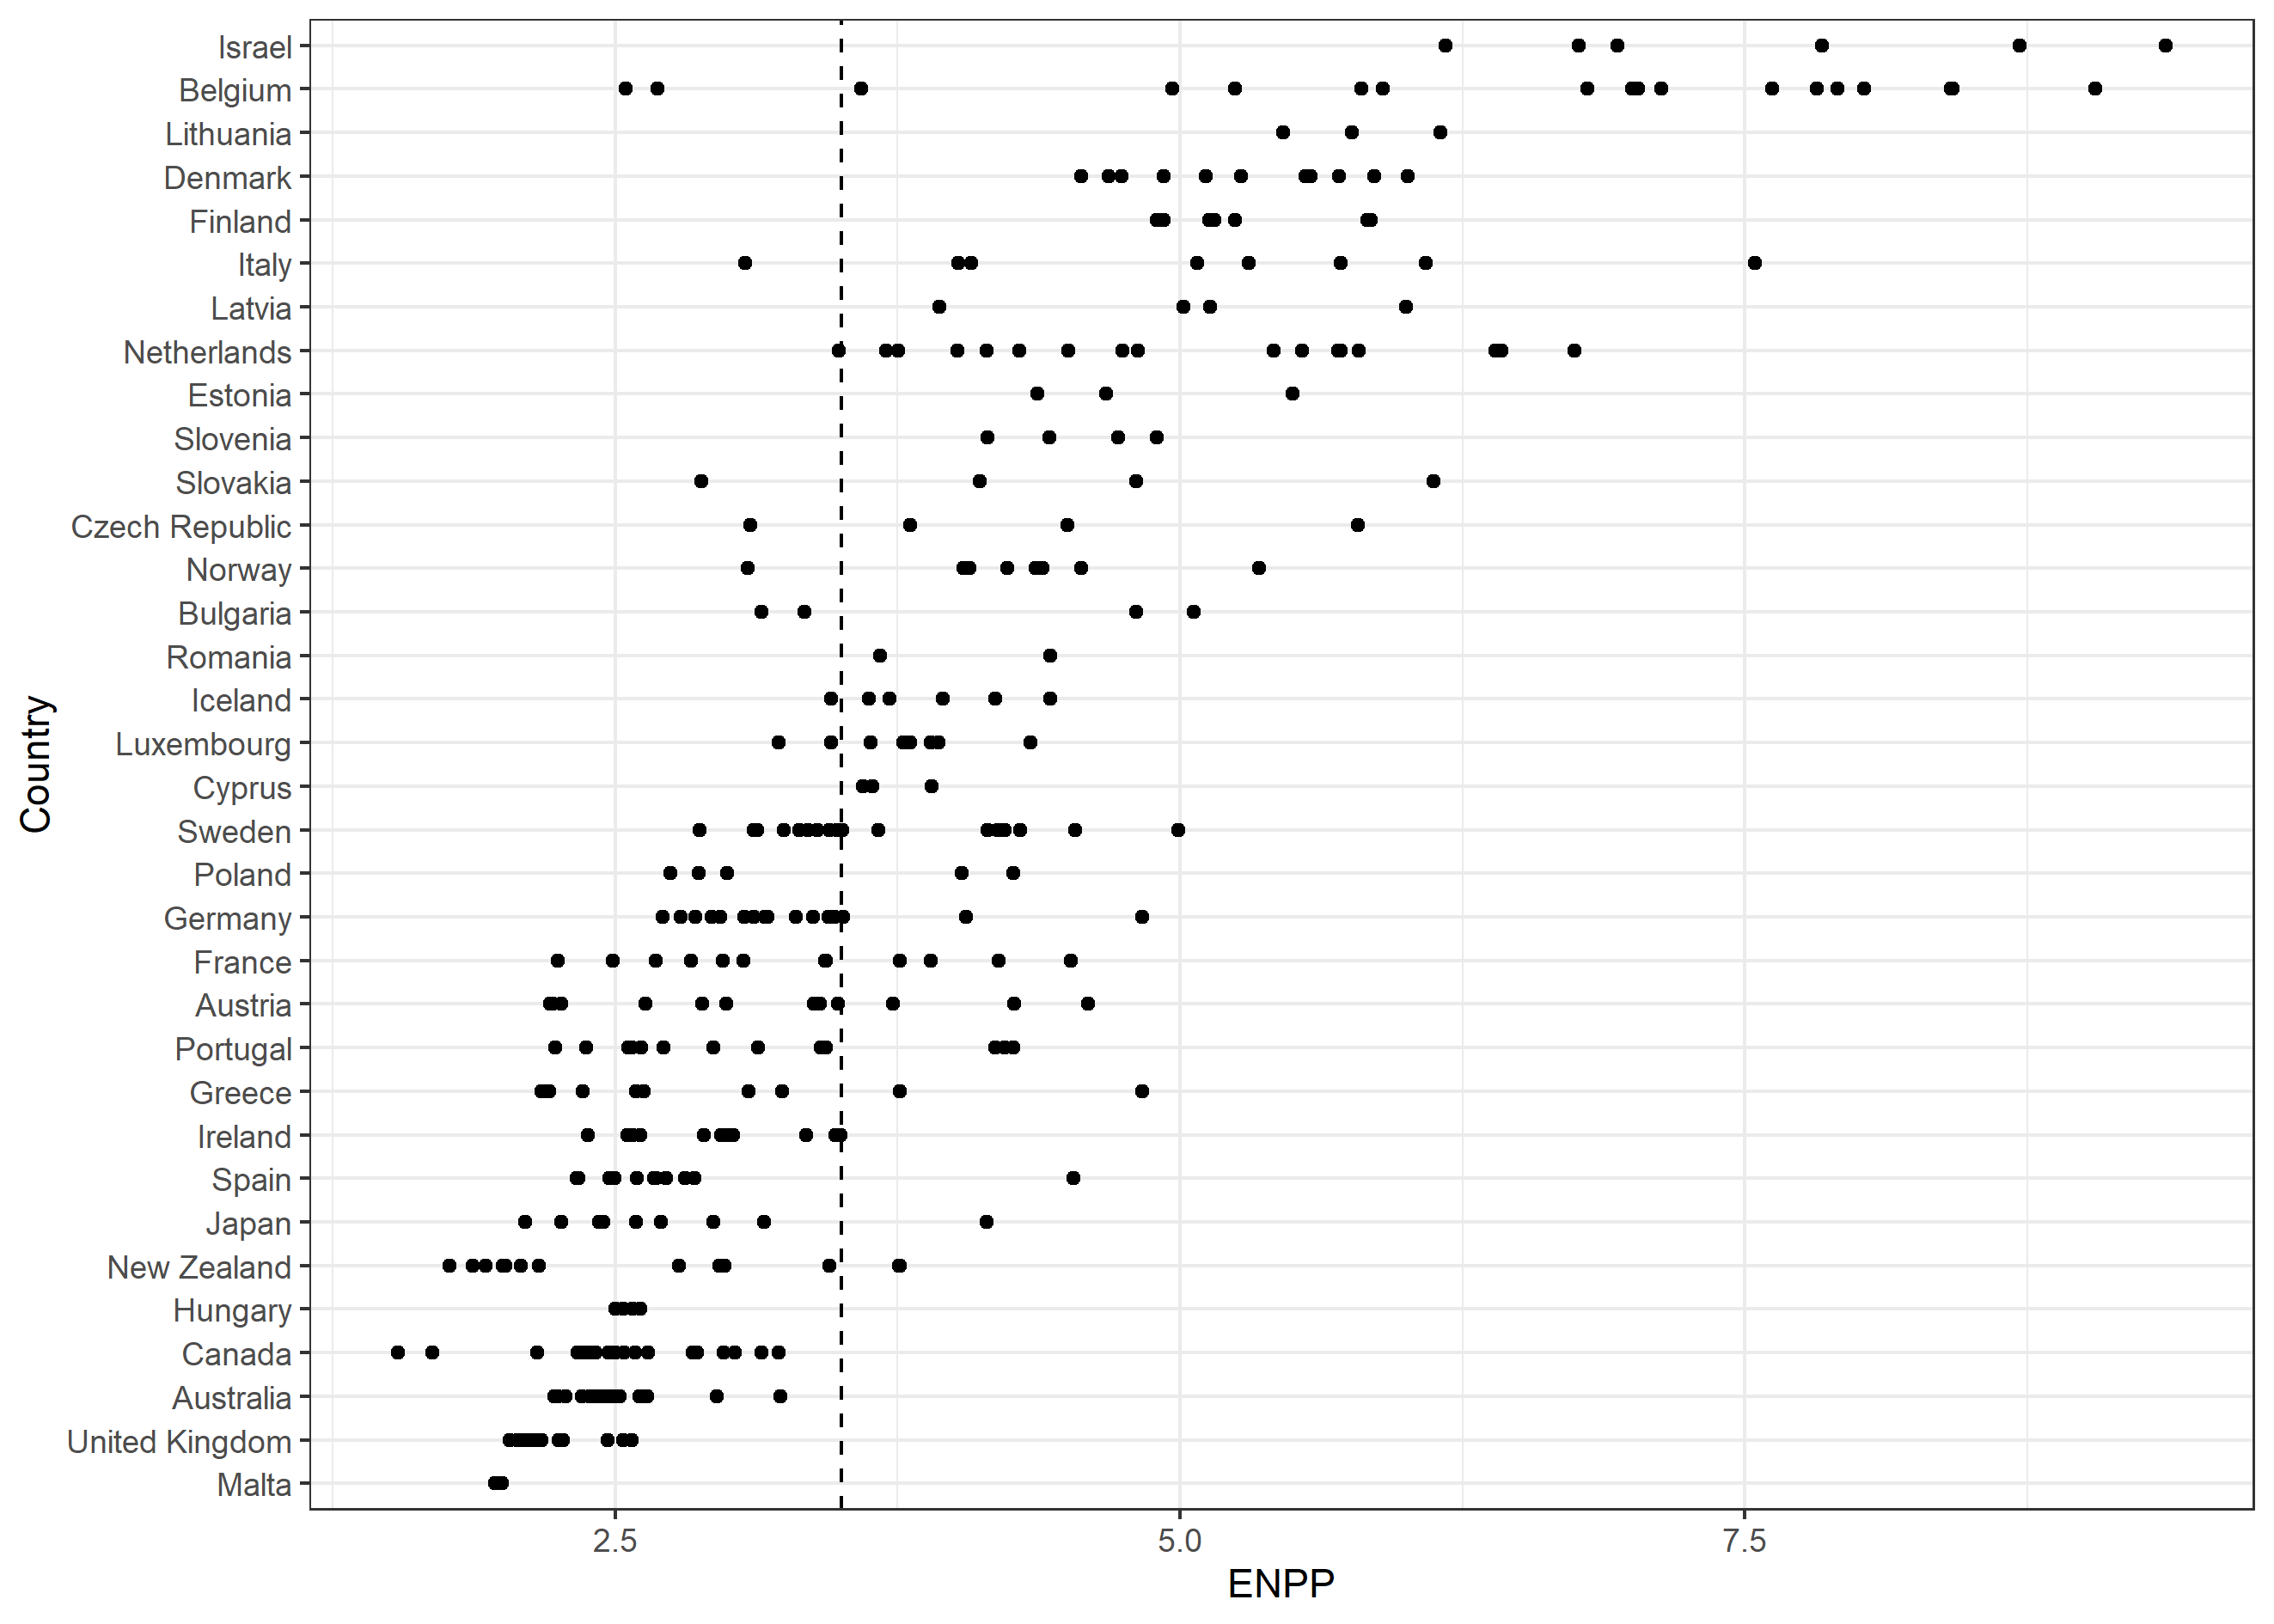
\includegraphics[width=\linewidth]{figures/Figure7.png}
		\caption{Party fragmentation in parliament by country-year. The dashed vertical line is our cutoff for classifying low vs. high fragmentation elections.}
		\label{fig:LowFragHighFrag}
	\end{figure}
    
	Figure \ref{fig:rdEstimateVaryingENPP} illustrates how the RD estimate and 95\% confidence interval changes when we vary the ENPP threshold. The result holds for cutoffs less than 3.5, though when it is less than 3 the effective sample size is much smaller, yielding larger robust standard errors. 
	
	\begin{figure}[h]
		\centering
		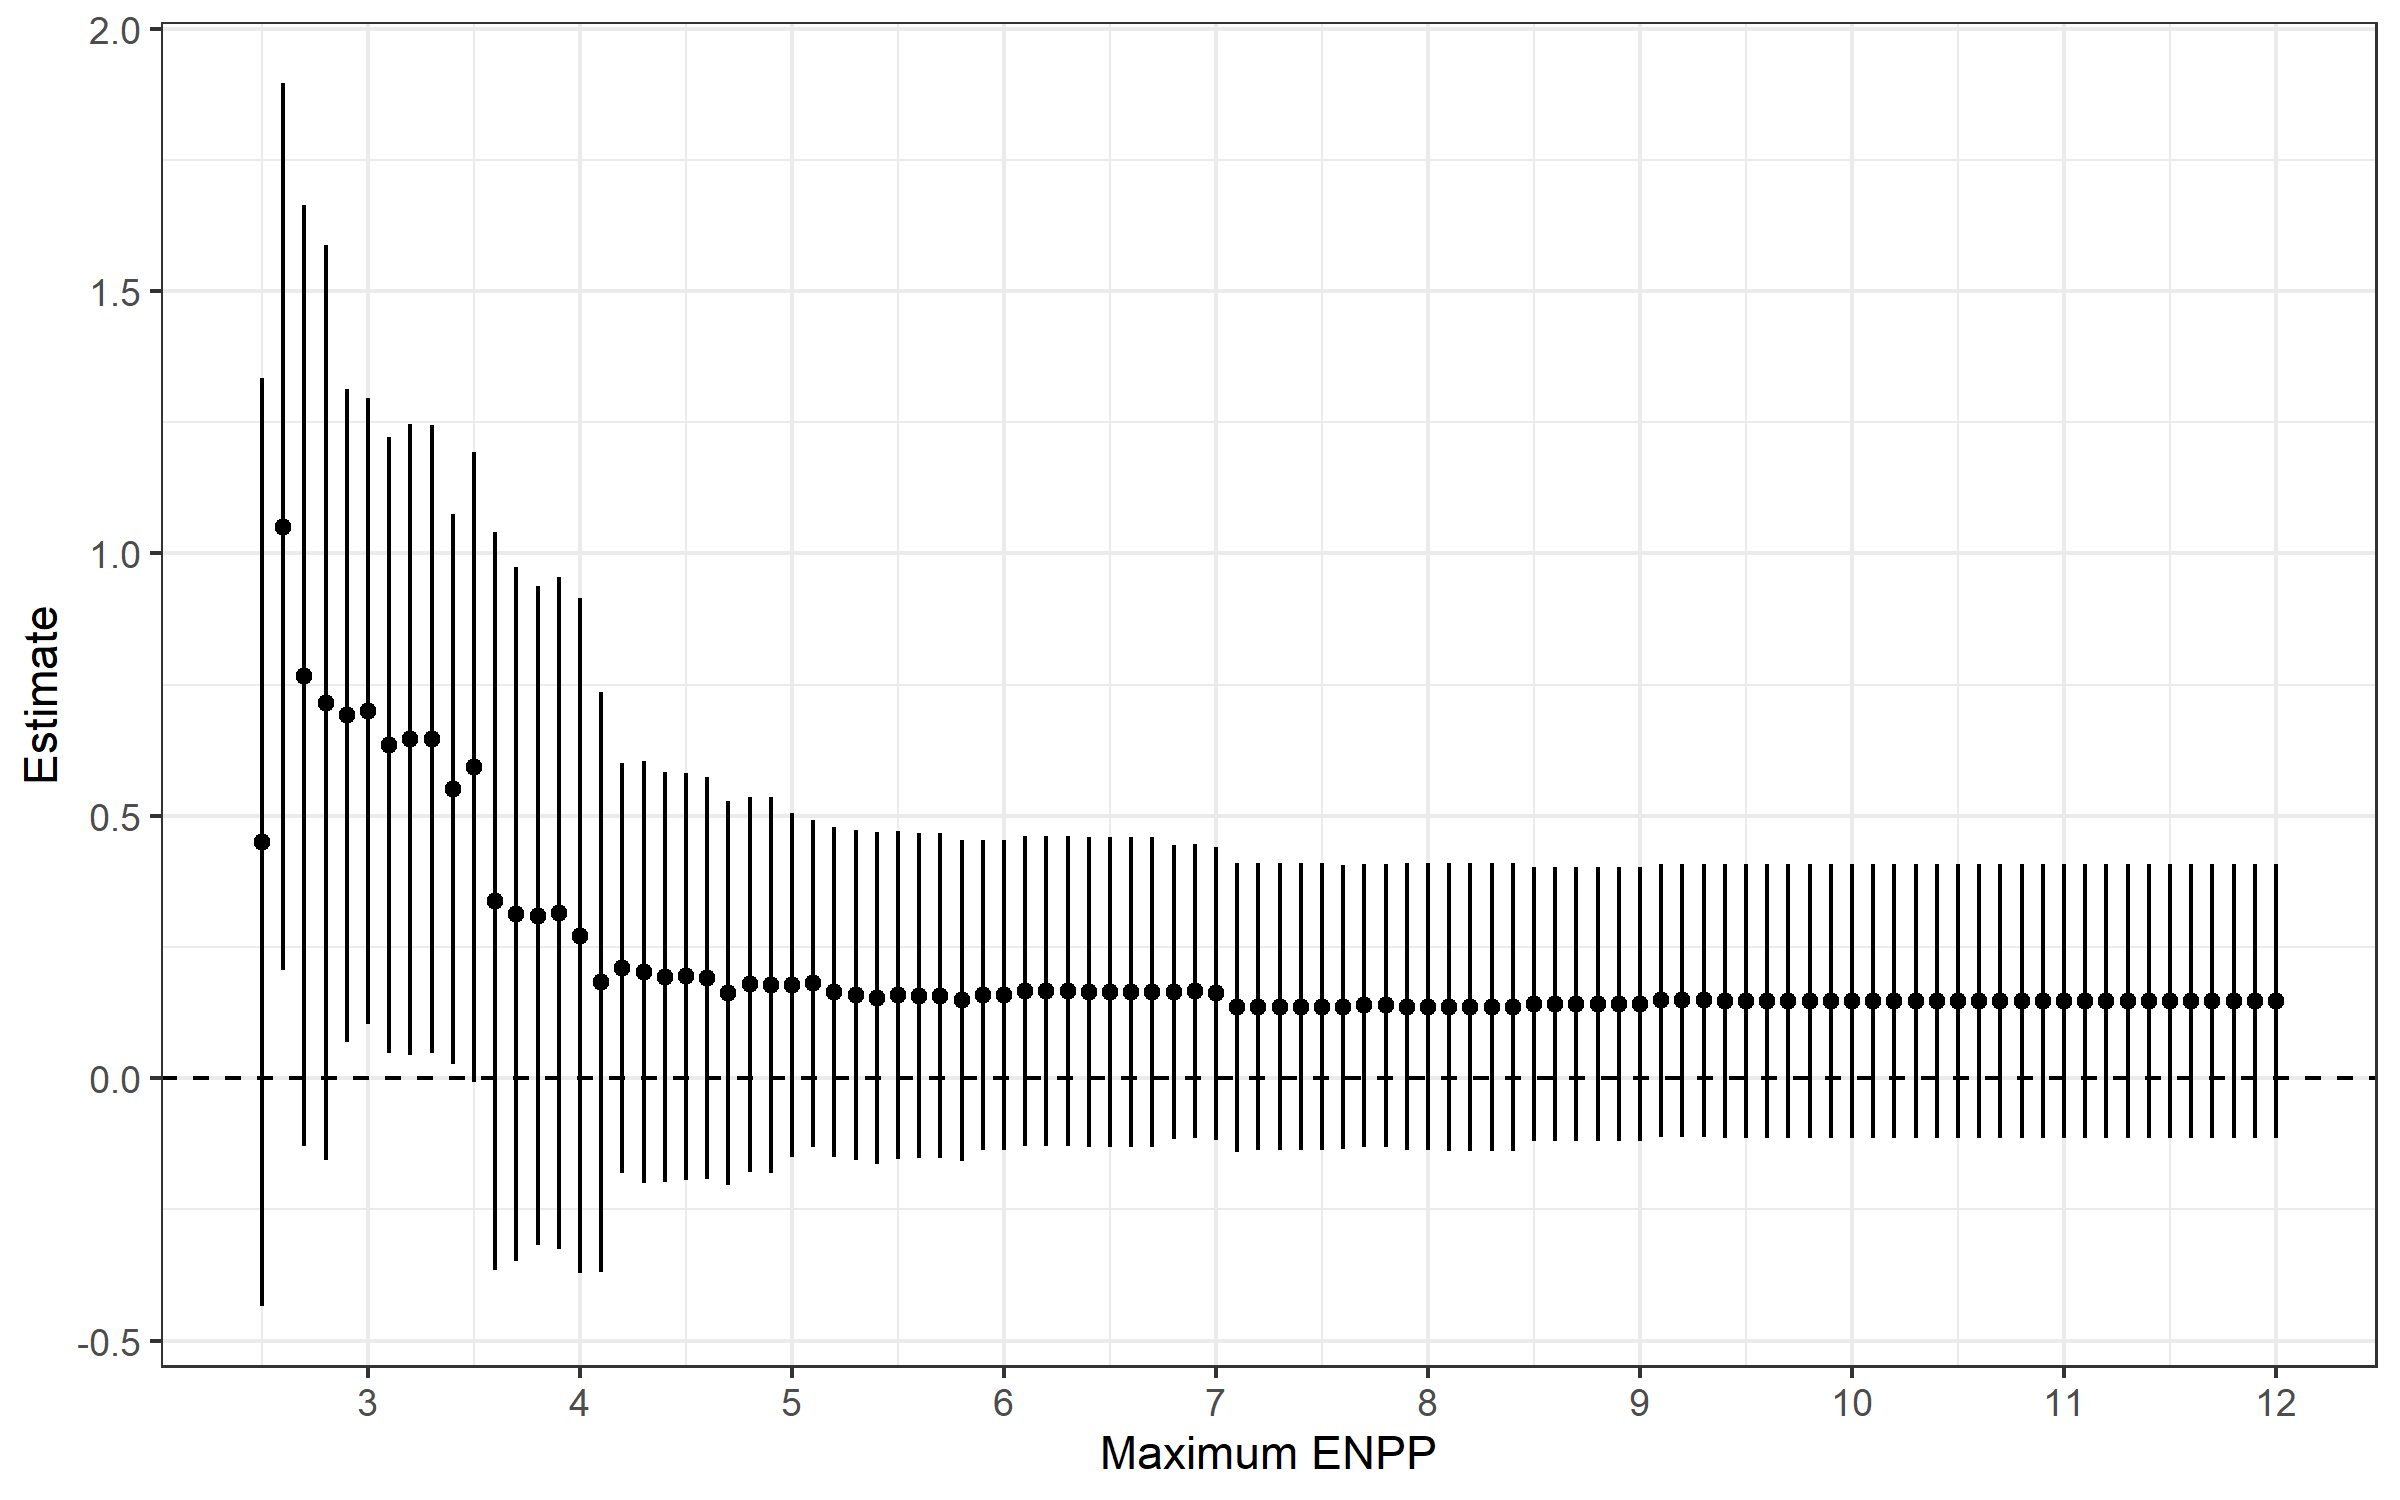
\includegraphics[width=\linewidth]{figures/Figure8.png}
		\caption{Estimated treatment effects and 95\% confidence intervals, varying the ENPP threshold. The estimate is largest when party fragmentation is low (ENPP $< 3.5$)}
		\label{fig:rdEstimateVaryingENPP}
	\end{figure}

	\subsection{Regression Discontinuity with Covariates}
	
	\citet{Calonico2018} propose a procedure to adjust for covariates in a regression discontinuity framework. Estimating using this procedure -- conditioning on GDP per capita, log population, expenditures per capita, tax revenue as a percentage of GDP, and inflation -- yields the results in Table \ref{table:RDWithCovariates}. 
	
	% Table created by stargazer v.5.2.2 by Marek Hlavac, Harvard University. E-mail: hlavac at fas.harvard.edu
	% Date and time: Fri, Nov 16, 2018 - 2:02:49 PM
	\begin{table}[h] \centering 
		\caption{Regression discontinuity with pre-treatment covariates. Dependent variable = 1-month bond yield regression discontinuity estimates (bias-corrected) with 95\% confidence intervals (robust standard errors) in brackets.} 
		\label{table:RDWithCovariates} 
		\begin{tabular}{@{\extracolsep{5pt}}lccc} 
			\\[-1.8ex]\hline 
			\hline \\[-1.8ex] 
			& \multicolumn{3}{c}{\textit{Fragmentation:}} \\ 
			\cline{2-4} 
			\\[-1.8ex] & All & Low & High \\ 
			\\[-1.8ex] & (1) & (2) & (3)\\ 
			\hline \\[-1.8ex] 
			Local Average Treatment Effect & 0.146 & 1.01 & $-0.146$ \\ 
			& [-0.14, 0.43] & [0.46, 1.56] & [-0.45, 0.16] \\ 
			\hline \\[-1.8ex] 
			Observations & 236 & 118 & 118 \\ 
			Bandwidth Estimate $(h)$ & 0.138 & 0.135 & 0.129 \\ 
			\hline 
			\hline \\[-1.8ex] 
		\end{tabular} 
	\end{table}  


	\subsection{Sensitivity to Bandwidth}
	
	As Figure \ref{fig:bandwidthSensitivity} illustrates, our result is somewhat sensitive to choice of bandwidth. Using a smaller bandwidth than the CCT optimum yields significantly fewer observations near the cutoff, increasing standard errors. And the local-linear estimate shrinks with larger bandwidths (as one would expect given the theoretical conditional expectation function presented in Section \ref{section:formal_model}). 
	
	
	\begin{figure}[h]
	\centering
	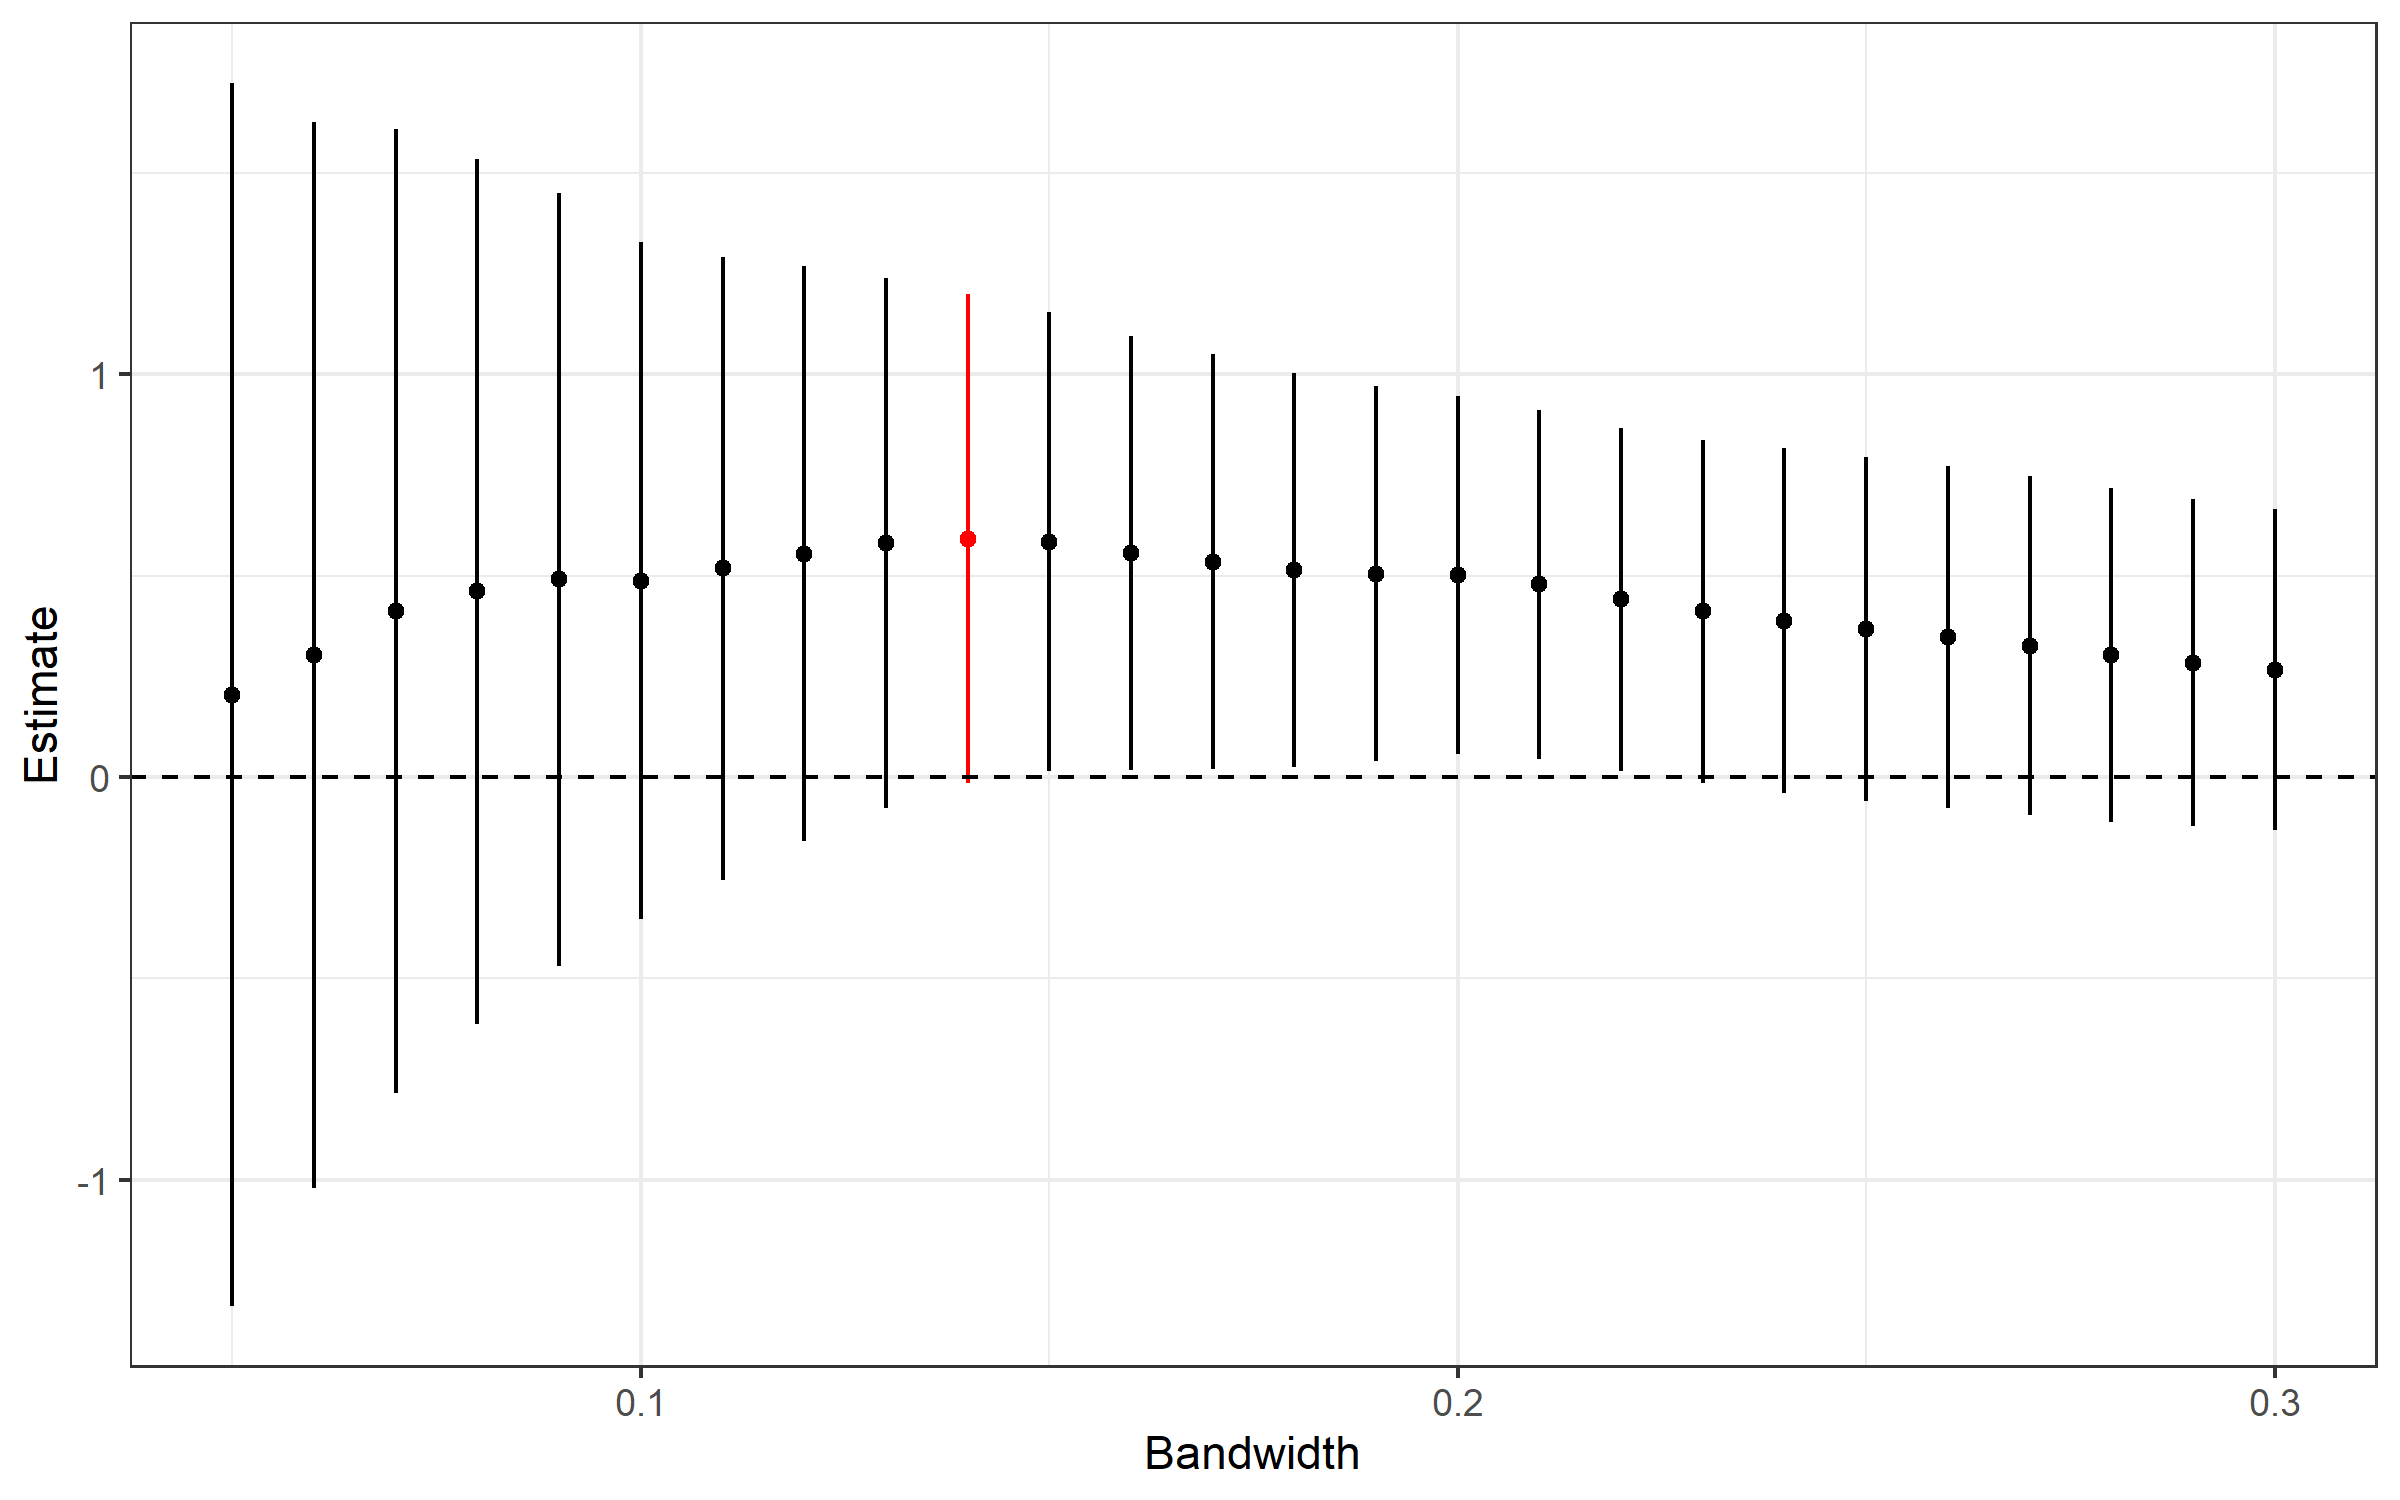
\includegraphics[width=\linewidth]{figures/Figure9.png}
	\caption{Sensitivity to choice of bandwidth. Bias-corrected estimates and 95\% confidence intervals (robust standard errors). The CCT optimal bandwidth is plotted in red.}
	\label{fig:bandwidthSensitivity}
	\end{figure}

	\subsection{Sensitivity to Polynomial Order and Kernel Function}

	The \texttt{rdrobust} package defaults to modeling the conditional expectation function with a local-linear and triangular kernel weights. The core result is robust to varying these assumptions, though the 95\% confidence interval is wider (and includes zero) when estimated using a second-order polynomial.
	 
	% Table created by stargazer v.5.2.2 by Marek Hlavac, Harvard University. E-mail: hlavac at fas.harvard.edu
	% Date and time: Fri, Nov 16, 2018 - 2:02:49 PM
	\begin{table}[h] \centering 
		\caption{Regression discontinuity estimates, varying polynomial order and kernel function. Dependent variable = 1-month bond yield regression discontinuity estimates (bias-corrected) with 95\% confidence intervals (robust standard errors) in brackets.} 
		\label{table:RDQuadratic} 
		\begin{tabular}{@{\extracolsep{5pt}}lccc} 
			\\[-1.8ex]\hline 
			\hline \\[-1.8ex] 
			& \multicolumn{3}{c}{\textit{Fragmentation:}} \\ 
			\cline{2-4} 
			\\[-1.8ex] & All & Low & High \\ 
			\\[-1.8ex] & (1) & (2) & (3)\\ 
			\hline \\[-1.8ex] 	
			Linear, Triangular Kernel & 0.145 & 0.592 & $-0.048$ \\ 
			& [-0.12, 0.43] & [-0.01, 1.19] & [-0.32, 0.23] \\ 
			Linear, Uniform Kernel & 0.152 & 0.511 & $-0.077$ \\ 
			& [-0.20, 0.39] & [0.10, 0.92] & [-0.39, 0.23] \\ 
			Quadratic, Triangular Kernel & 0.099 & 0.646 & $-0.109$ \\ 
			& [-0.20, 0.39] & [$-0.11$, 1.40] & [-0.43, 0.21] \\ 
			Quadratic, Uniform Kernel & 0.106 & 0.598 & 0.016 \\ 
			& [-0.19, 0.41] & [$-0.14$, 1.33] & [-0.31, 0.34] \\ 
			\hline \\[-1.8ex] 
			Observations & 316 & 179 & 137 \\ 
			%Bandwidth Estimate $(h)$ & 0.203 & 0.241 & 0.152 \\ 
			\hline 
			\hline \\[-1.8ex] 
		\end{tabular} 
	\end{table}  
	
	\subsection{Dynamic RD Estimates} 

        In addition to estimating the short-run effects on bond yields, we can compute a dynamic RD estimate -- actually a series of static estimates -- by varying the time window with which the dependent variable is measured \citep{Cellini2010}. Using this method, we can observe whether a left party plurality yields longer-term changes to bond yields. Furthermore, as a placebo test, we can also examine whether there is an estimated effect on bond yields \textit{prior} to the election. Figure \ref{fig:dynamicRD} illustrates the results from this moving-window RD analysis; the narrow plurality win of a left party appears to have an effect on bond yields that persist for at least a year, peaking at around 10 months, when party fragmentation is low, and, again, no perceptible effect at any time-window in high-fragmentation contexts. 

    \begin{figure} [h]
    	\centering
    	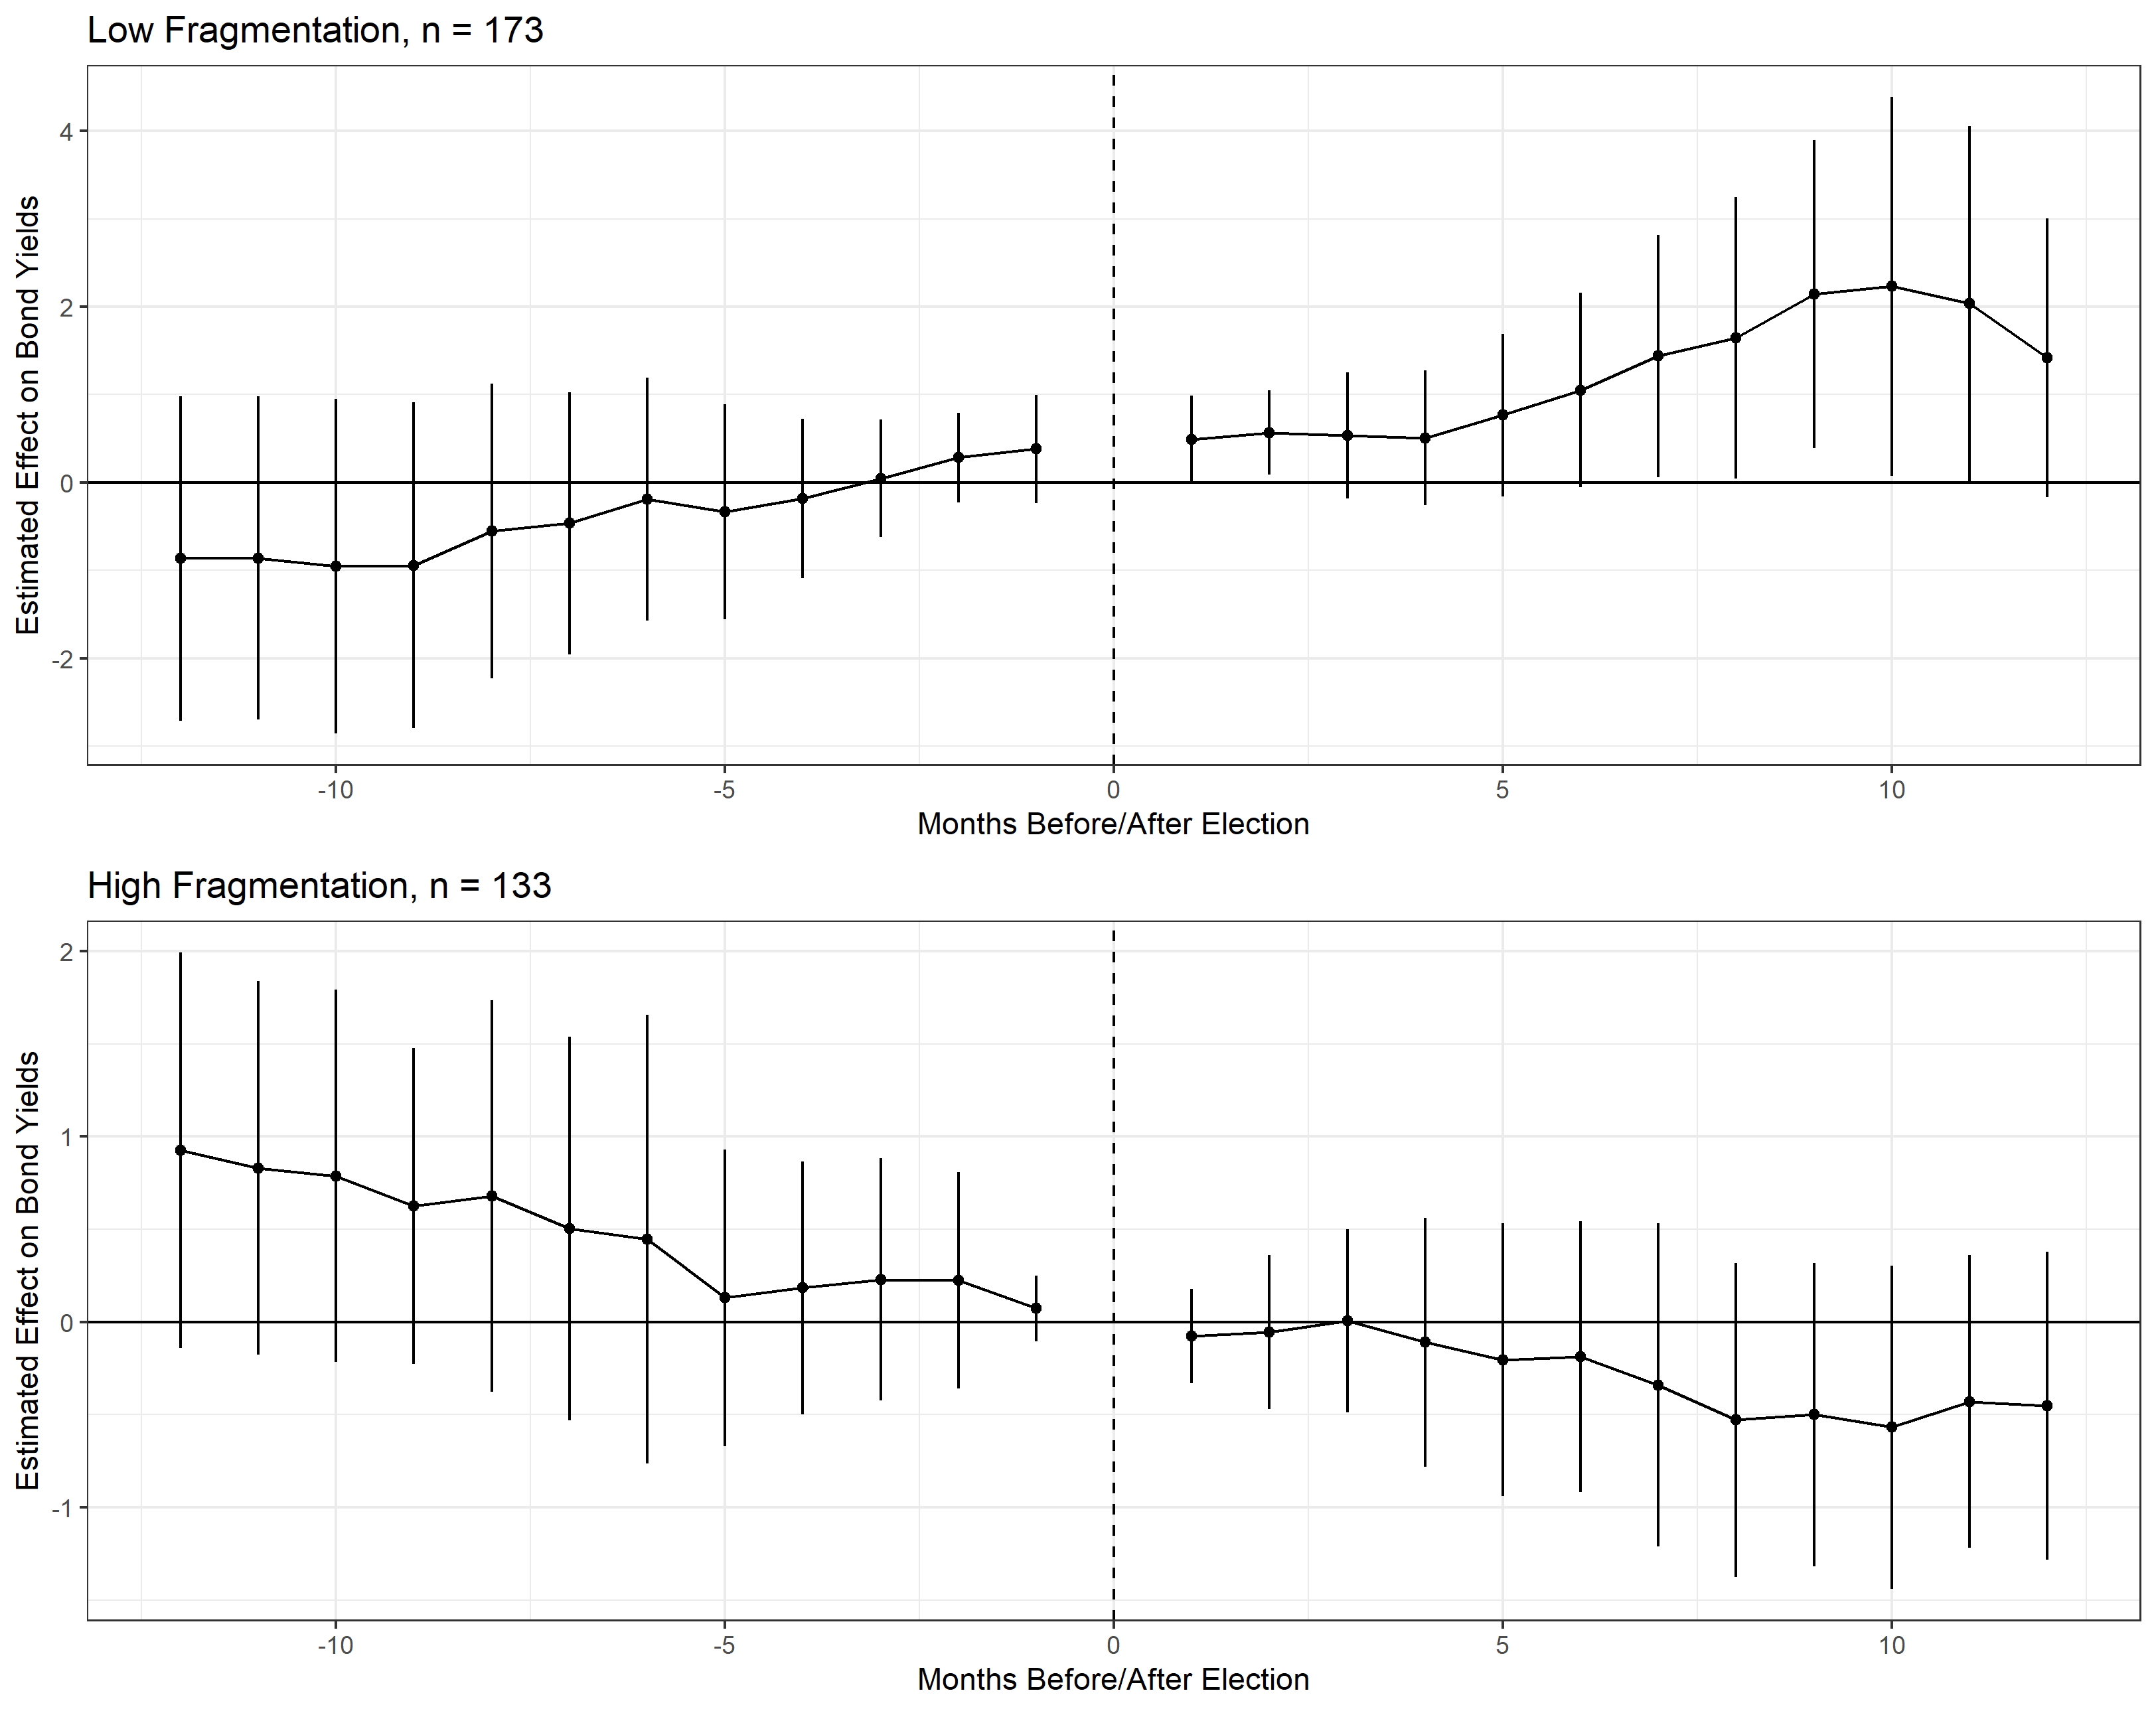
\includegraphics[width=\linewidth]{figures/Figure10.png}
    	\caption{Dynamic RD estimates. Top panel is for low fragmentation elections ($ENPP < 3.5$), bottom panel is for high fragmentation elections ($ENPP > 3.5$).}
    	\label{fig:dynamicRD}
    \end{figure}

\end{appendices}





\end{document}